\documentclass[a4paper]{article}
\usepackage[normalem]{ulem}
\usepackage{eurosym}
\usepackage[font=small,labelfont=bf]{caption}

% impostazioni generali
%Tutti gli usepackage vanno qui
\usepackage{geometry}
\usepackage[italian]{babel}
\usepackage[utf8]{inputenc}
\usepackage{tabularx}
\usepackage{longtable}
\usepackage{hyperref}
\usepackage{enumitem}
\usepackage{array} 
\usepackage{booktabs}
\newcolumntype{M}[1]{>{\centering\arraybackslash}m{#1}}
\usepackage[toc]{appendix}
\usepackage{caption}

\hypersetup{
	colorlinks=true,
	linkcolor=blue,
	filecolor=magenta,
	urlcolor=blue,
}
% Numerazione figure
\let\counterwithout\relax
\let\counterwithin\relax
\usepackage{chngcntr}

% distanziare elenco delle figure e delle tabelle
\usepackage{tocbasic}
\DeclareTOCStyleEntry[numwidth=3.5em]{tocline}{figure}% for figure entries
\DeclareTOCStyleEntry[numwidth=3.5em]{tocline}{table}% for table entries


%\counterwithout{table}{section}
%\counterwithout{figure}{section}
\captionsetup[table]{font=small,skip=5pt} 

\usepackage[bottom]{footmisc}
\usepackage{fancyhdr}
\setcounter{secnumdepth}{4}
\usepackage{amsmath, amssymb}
\usepackage{array}
\usepackage{graphicx}

\usepackage{ifthen}

\usepackage{float}
\restylefloat{table}

\usepackage{layouts}
\usepackage{url}
\usepackage{comment}
\usepackage{eurosym}

\usepackage{lastpage}
\usepackage{layouts}
\usepackage{eurosym}

\geometry{a4paper,top=3cm,bottom=4cm,left=2.5cm,right=2.5cm}

%Comandi di impaginazione uguale per tutti i documenti
\pagestyle{fancy}
\lhead{
\includegraphics[scale=0.05]{../../../template/images/logo.png}}
%Titolo del documento
\rhead{\doctitle{}}
%\rfoot{\thepage}
\cfoot{Pagina \thepage\ di \pageref{LastPage}}
\setlength{\headheight}{41pt}
\setcounter{tocdepth}{5}
\setcounter{secnumdepth}{5}
\renewcommand{\footrulewidth}{0.4pt}

% multirow per tabelle
\usepackage{multirow}

% Permette tabelle su più pagine
%\usepackage{longtable}


% colore di sfondo per le celle
\usepackage[table]{xcolor}

%COMANDI TABELLE
\newcommand{\rowcolorhead}{\rowcolor[HTML]{007c95}}
\newcommand{\captionline}{\rowcolor[HTML]{FFFFFF}} %comando per le caption delle tabelle
\newcommand{\cellcolorhead}{\cellcolor[HTML]{007c95}}
\newcommand{\hlinetable}{\arrayrulecolor[HTML]{007c95}\hline}

%intestazione
% check for missing commands
\newcommand{\headertitle}[1]{\textbf{\color{white}#1}} %titolo colonna
\definecolor{pari}{HTML}{b1dae3}
\definecolor{dispari}{HTML}{d7f2f7}

% comandi \textit{Glossario}
\newcommand{\glo}{$_{G}$}
\newcommand{\glosp}{$_{G}$ }


%label custom
\makeatletter
\newcommand{\uclabel}[2]{%
	\protected@write \@auxout {}{\string \newlabel {#1}{{#2}{\thepage}{#2}{#1}{}} }%
	\hypertarget{#1}{#2}
}
\makeatother

%riportare pezzi di codice
\definecolor{codegray}{gray}{0.9}
\newcommand{\code}[1]{\colorbox{codegray}{\texttt{#1}}}

%versioni documenti
\newcommand{\AdRversione}{1.0.0}
\newcommand{\NdPversione}{1.0.0}
\newcommand{\PdPversione}{1.0.0}
\newcommand{\PdQversione}{1.0.0}
\newcommand{\Gloversione}{1.0.0}
\newcommand{\Stversione}{0.1.2}
\newcommand{\MUversione}{0.1.0}
%nome documento con versione 
\newcommand{\AdRdocumento}{\textit{Analisi dei Requisiti v.\AdRversione} }
\newcommand{\NdPdocumento}{\textit{Norme di Progetto v.\NdPversione} }
\newcommand{\PdPdocumento}{\textit{Piano di Progetto v.\PdPversione} }
\newcommand{\PdQdocumento}{\textit{Piano di Qualifica v.\PdQversione} }
\newcommand{\Glodocumento}{\textit{Glossario v.\Gloversione} }
\newcommand{\Stdocumento}{\textit{Glossario v.\Stversione} }
\newcommand{\MUDocumento}{\textit{Glossario v.\MUversione} }

% dati della prima pagina
% Configurazione della pagina iniziale
\newcommand{\doctitle}{\textit{Glossario}}
\newcommand{\rev}{0.3.1} % versione
\newcommand{\resp}{Ibra Elton} % inserire responsabile
\newcommand{\red}{Corbu Teodor Mihail}
\newcommand{\ver}{Andreetto Alessio}
\newcommand{\uso}{Esterno}
\newcommand{\dest}{\textit{Project Origin}
	\\ Prof. Vardanega Tullio 
	\\ Prof. Cardin Riccardo}
\newcommand{\describedoc}{Glossario contenente i termini per i quali è necessaria una definizione univoca del gruppo \newline \textit{Project Origin} nella realizzazione del progetto \textit{Personal Identity Wallet}}

 % per modificare la prima pagina editare questo file

\makeindex

\makeatletter
\renewcommand\paragraph{
\@startsection {paragraph}{4}{0mm}{-\baselineskip}{.5\baselineskip}{\normalfont \normalsize \bfseries }}
\makeatother

\begin{document}

% Prima pagina
\thispagestyle{empty}
\renewcommand{\arraystretch}{1.3}

\begin{titlepage}
	\begin{center}
		
	
\includegraphics[scale = 0.20]{../../../template/images/logo.png}
	\\[1cm]
	\href{mailto:projectorigin2023@gmail.com}		      	
	{\large{\textit{projectorigin2023@gmail.com} } }\\[2.5cm]
	\Huge \textbf{\doctitle} \\[1cm]
	 \large
			 \begin{tabular}{r|l}
                        \textbf{Versione} & \rev{} \\
                        \textbf{Responsabile} & \resp{} \\
                        \textbf{Redattori} & \red{} \\ 
                        \textbf{Verificatori} &  \ver{} \\
                        \textbf{Uso} & \uso{} \\                        
                        \textbf{Destinatari} & \parbox[t]{5cm}{ \dest{} }
                \end{tabular} 
                \\[3.3cm]
                \large \textbf{Descrizione} \\ \describedoc{} 
     \end{center}
\end{titlepage}

% Diario delle modifiche
\section*{Registro delle modifiche}

\newcommand{\changelogTable}[1]{
	 

\renewcommand{\arraystretch}{1.5}
\rowcolors{2}{pari}{dispari}
\begin{longtable}{ 
		>{\centering}M{0.07\textwidth} 
		>{\centering}M{0.13\textwidth}
		>{\centering}M{0.20\textwidth}
		>{\centering}M{0.17\textwidth} 
		>{\centering\arraybackslash}M{0.30\textwidth} 
		 }
	\rowcolorhead
	\headertitle{Vers.} &
	\centering \headertitle{Data} &	
	\headertitle{Autore} &
	\headertitle{Ruolo} & 
	\headertitle{Descrizione} 
	\endfirsthead	
	\endhead
	
	#1

\end{longtable}
\vspace{-2em}

}

\changelogTable{
    0.1.0 & 2023-05-11 & Corbu Teodor \\Bobirica Andrei& Verificatore & Verifica documento\\
    0.0.1 & 2023-05-11 & Beschin Michele & Analista & Stesura iniziale documento\\
} % editare questo
\pagebreak


% Indice
{
    \hypersetup{linkcolor=black}
    \tableofcontents
}
\pagebreak

% sezioni comuni 
% Informazioni generali
% \setcounter{table}{0} forse questo serve se l'indice delle tabelle parte da numeri sospetti
\section{Introduzione}

\subsection{Scopo de documento}
L’obiettivo del presente documento è di fornire una stima dei costi e dei tempi di consegna del progetto, nonché un piano dettagliato corredato di orari per ogni ruolo coinvolto. \\
La pianificazione sarà basata sull’analisi periodica delle attività svolte e una retrospettiva su quelle attività già completate, al fine di mantenere aggiornate e valide le 
stime effettuate. \\ Nel documento vengono inoltre identificate le possibili problematiche che il team potrebbe incontrare durante l’intero periodo di svolgimento del progetto.

\subsection{Scopo del prodotto}
Il capitolato prevede la realizzazione di un sistema di autenticazione dove un ente rilascia certificati di identità ad un utente, essi vengono memorizzati in un \textit{wallet}, 
per poi essere utilizzati per accedere a servizi. Sono previsti tre attori:
\begin{itemize}
    \item \textbf{Emittente}: entità che rilascia i certificati;
    \item \textbf{Holder}: persona fisica, che memorizza le credenziali di identità all'interno di un wallet;
    \item \textbf{Verifier}: entità che richiede delle credenziali per accedere a dei servizi.
\end{itemize}

\subsection{Glossario}
Al fine di evitare dubbi e ambiguità per determinati termini viene fornito un \textit{Glossario} che riporta la definizione specifica dei suddetti termini. 
Essi verranno contrassegnati con una lettera G (esempio\textsubscript{g}) a fine della parola. 
Tali termini verranno contrassegnati una sola volta per paragrafo onde evitare fastidiose ripetizioni. 

\subsection{Riferimenti}

\subsubsection{Riferimenti normativi}
\begin{itemize}
    \item \textit{Norme di progetto}: v 0.0.1
    \item Regolamento del progetto didattico: \\
    \url{https://www.math.unipd.it/~tullio/IS-1/2022/Dispense/PD02.pdf}
\end{itemize}

\subsubsection{Riferimenti informativi}
\begin{itemize}
    \item \textit{Analisi dei requisiti}: v 0.0.1
    \item Presentazione capitolato C3 \textit{Personal Identity Wallet} \\ \url{https://www.math.unipd.it/~tullio/IS-1/2022/Progetto/C3.pdf}
    \item Gestione di Progetto - slide T4 del corso Ingegneria del Software \\ \url{https://www.math.unipd.it/~tullio/IS-1/2022/Dispense/T04.pdf}
\end{itemize}


\newpage %forse si può togliere il newpage
\section{Strumenti Necessari}
Per poter avviare il progetto occorre avere installato i seguenti programmi:
\begin{itemize}
   \item  Brew (versione minima 4.1.11);
   \item  npm (versione minima 9.8.1);
   \item  Nodejs (versione minima v20.6.1)
   \item  Docker (versione 20.10.24, oppure 24.0.6 o successivi)
   \item Docker Compose (versione 1.29.2-1)
\end{itemize}
Inoltre bisogna avere i permessi di amministratore del proprio computer



\subsection{Credenziali di accesso necessarie per il progetto}
Le credenziali utili per il progetto sono:
\begin{itemize}
   \item Database per Origin Wallet: User: admin, Host: 10.5.0.33, Database: originwallet, Password: admin, Port: 5432
   \item Database per origin issuer: User:admin, Host:10.5.0.31, Database:originissuer, Password: admin, Port:5432
   \item Utente Origin Issuer: email mario.rossi@gmail.com, password Mariorossi123!
   \item Utente Sysadmin Origin Issuer: email: ADMIN@admin.com password: ADmin1234?
\end{itemize}

\subsection{Requisiti minimi}
Per poter avviare il progetto occorre avere, sulla propria macchina, queste specifiche minime:
\begin{itemize}
   \item processore i5 2.7Ghz;
   \item 8GB di memoria RAM;
   \item 100GB memoria SSD
   \item sistema operativo Ubuntu, Linux (versione 22), oppure MacOS versione I5 (potrebbe dare problemi con la versione M1)
\end{itemize}
Le specifiche minime consigliate sono:
\begin{itemize}
   \item processore i7 2.7Ghz;
   \item 12GB di memoria RAM;
   \item 100GB memoria SSD
   \item sistema operativo Ubuntu, Linux (versione 22), oppure MacOS versione I5 (potrebbe dare problemi con la versione M1)
\end{itemize}

\subsection{Deploy del sistema}

Script di avvio:
\begin{itemize}
   \item git clone https://github.com/Project-Origin-2023/Personal-Identity-Wallet
   \item cd scripts
   \item sh deploy.sh
   \item inserire la password di sistema
   \item attendere completamento
\end{itemize}\newpage
\section{Issuer}

\subsection{Registrazione}
In questa sezione un utente può registarsi inserendo \textbf{Email} e \textbf{Password} valide. Una volta registrato l'utente riceverà un messaggio di conferma e verrà reindirizzato alla pagina \textbf{Home}.
\begin{center}
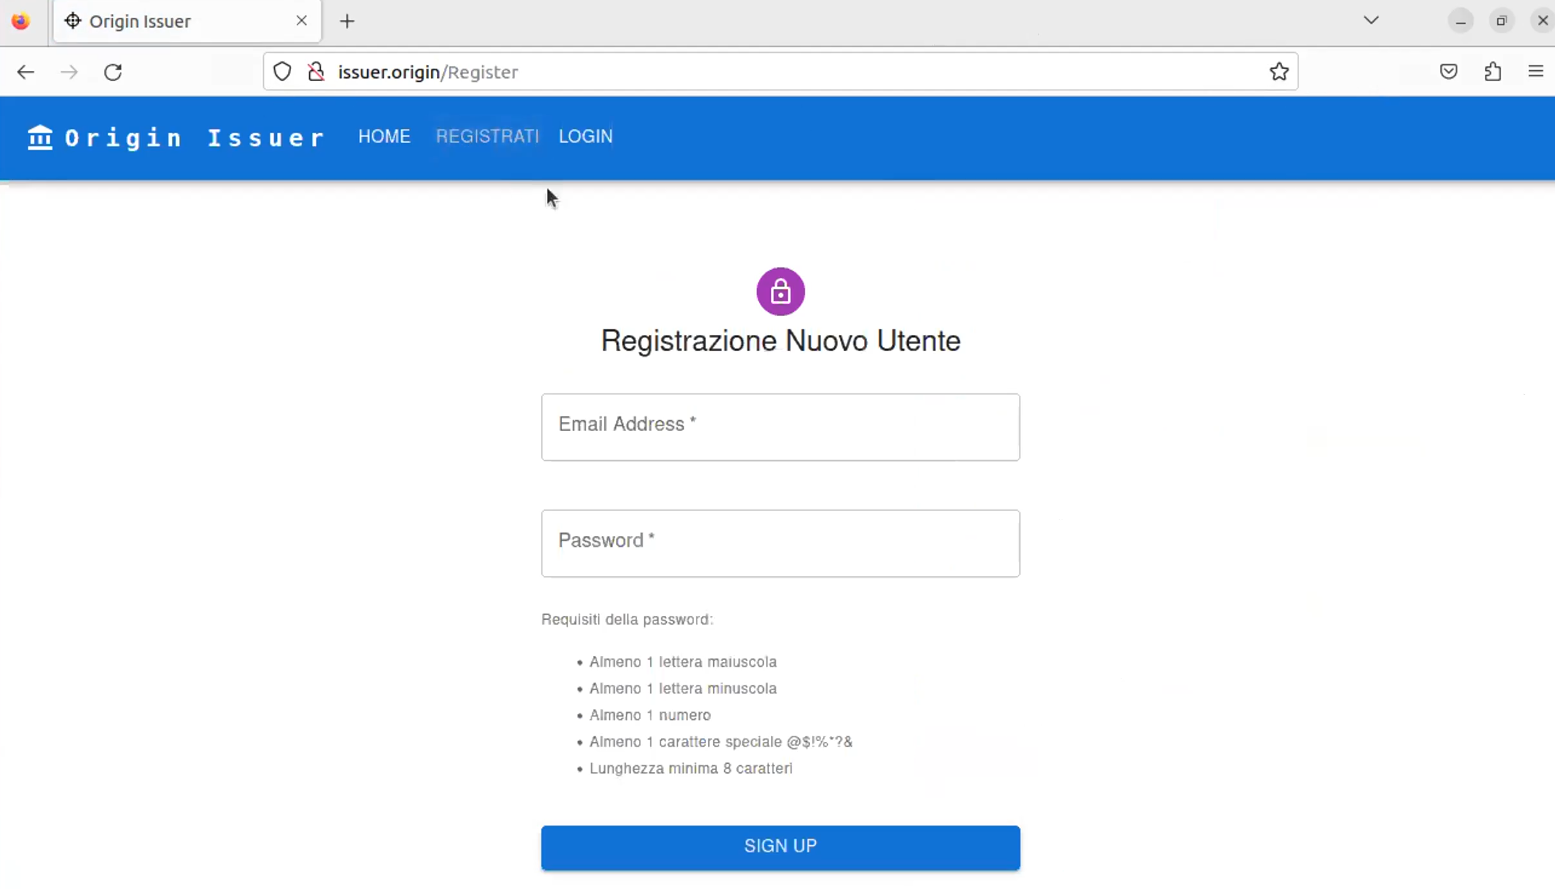
\includegraphics[scale = 0.2]{./res/img/issuer/new/registrazione.png}
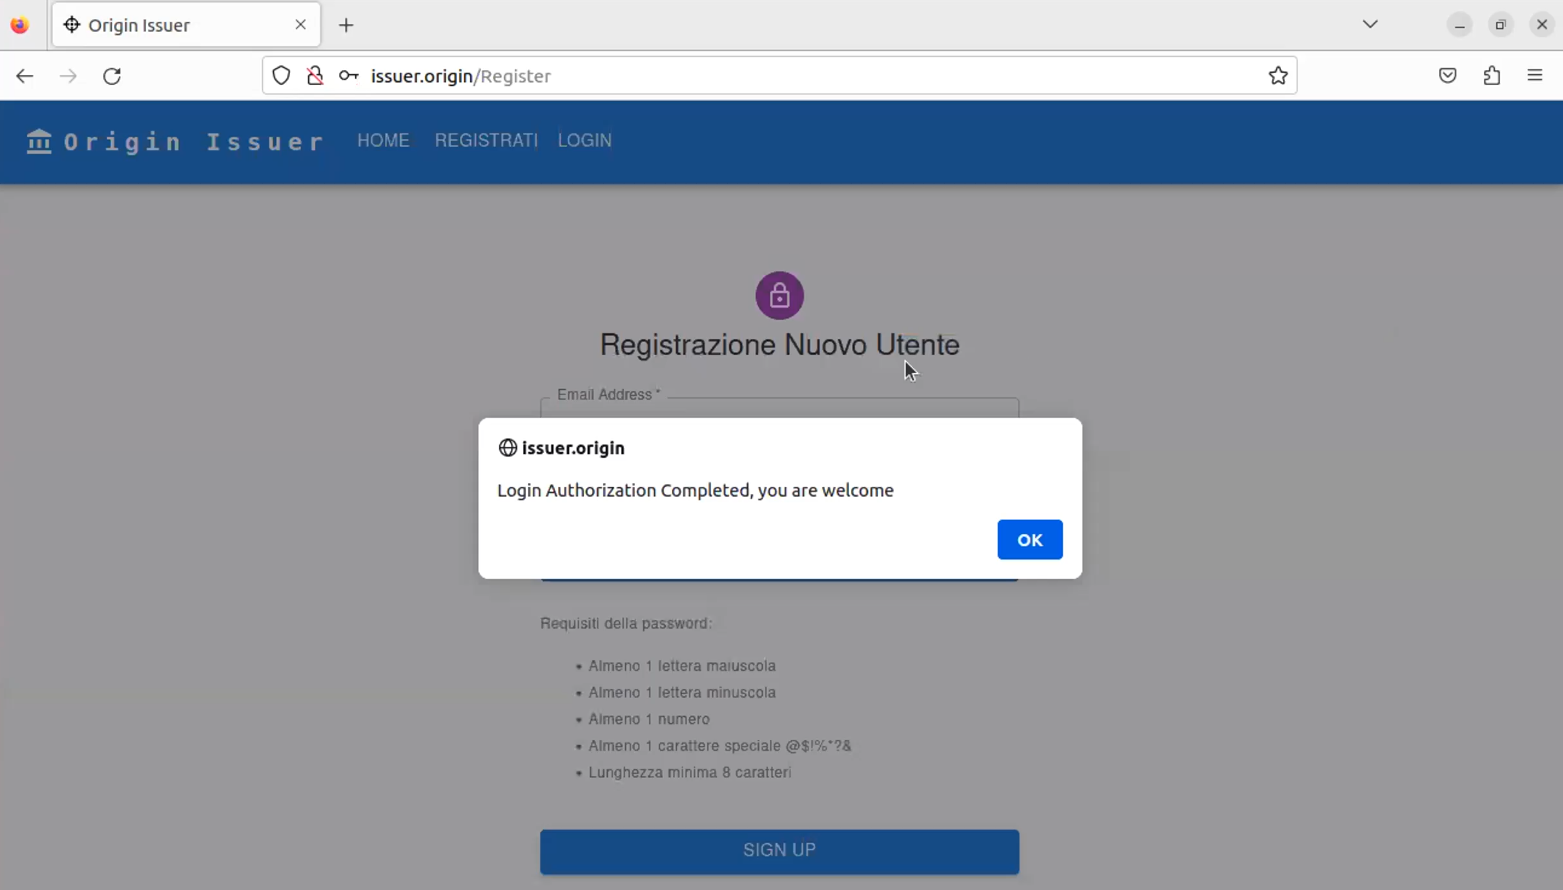
\includegraphics[scale = 0.2]{./res/img/issuer/new/registrazione2.png}
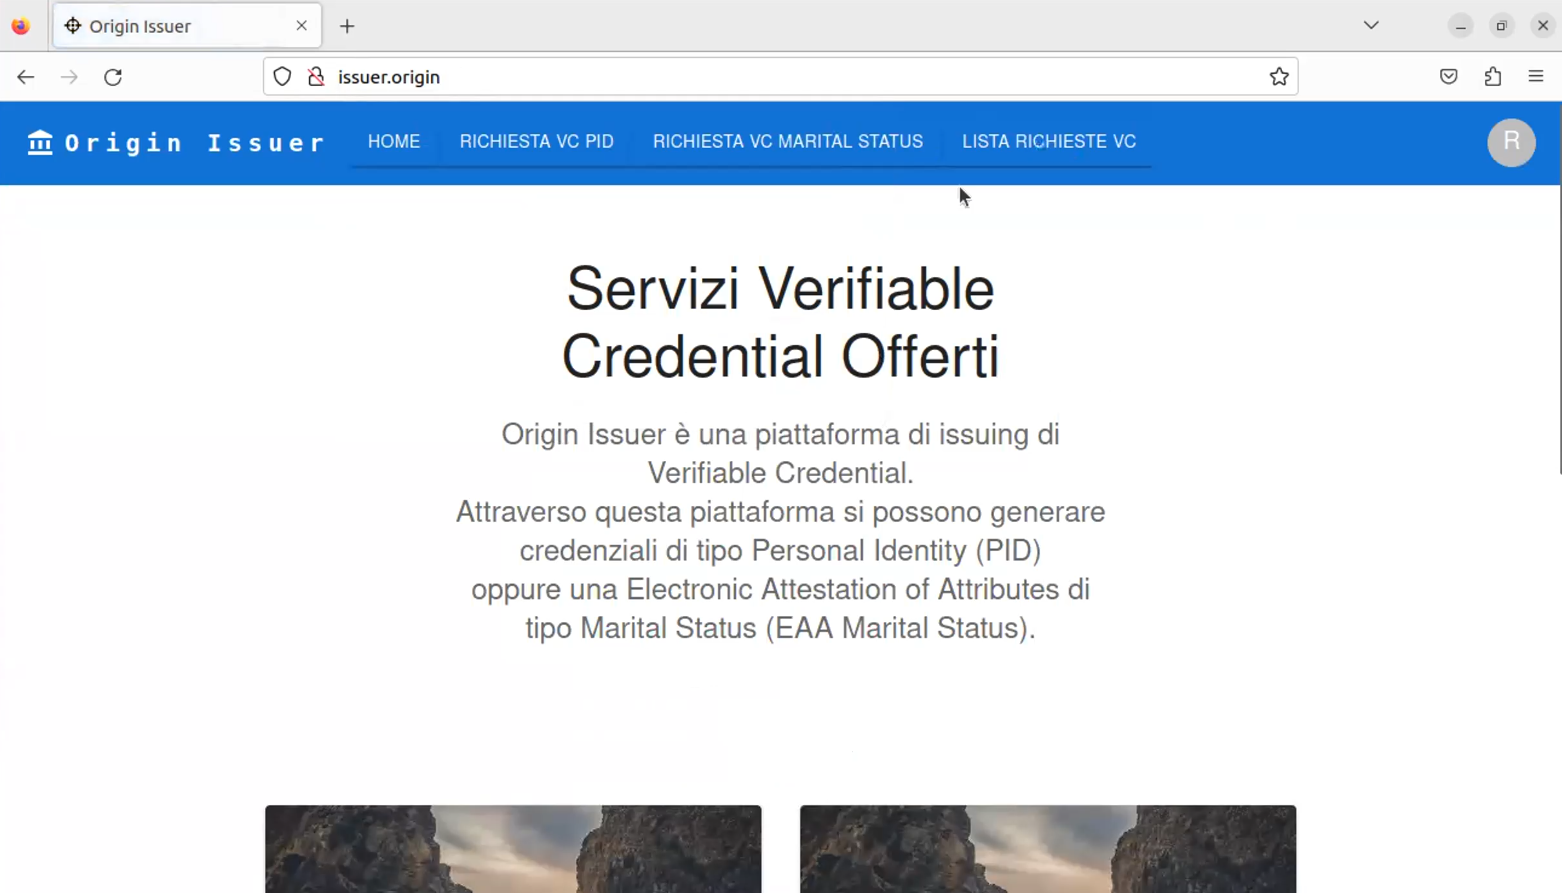
\includegraphics[scale = 0.2]{./res/img/issuer/new/registrazione3.png}
\end{center}

\subsection{Login}
\subsubsection{Login utente}
In questa pagina un \textbf{utente} può effettuare il login inserendo \textbf{Email} e \textbf{Password} valide. Una volta effettuato il login l'utente verrà reindirizzato alla sua pagina \textbf{Home}.
\begin{center}
    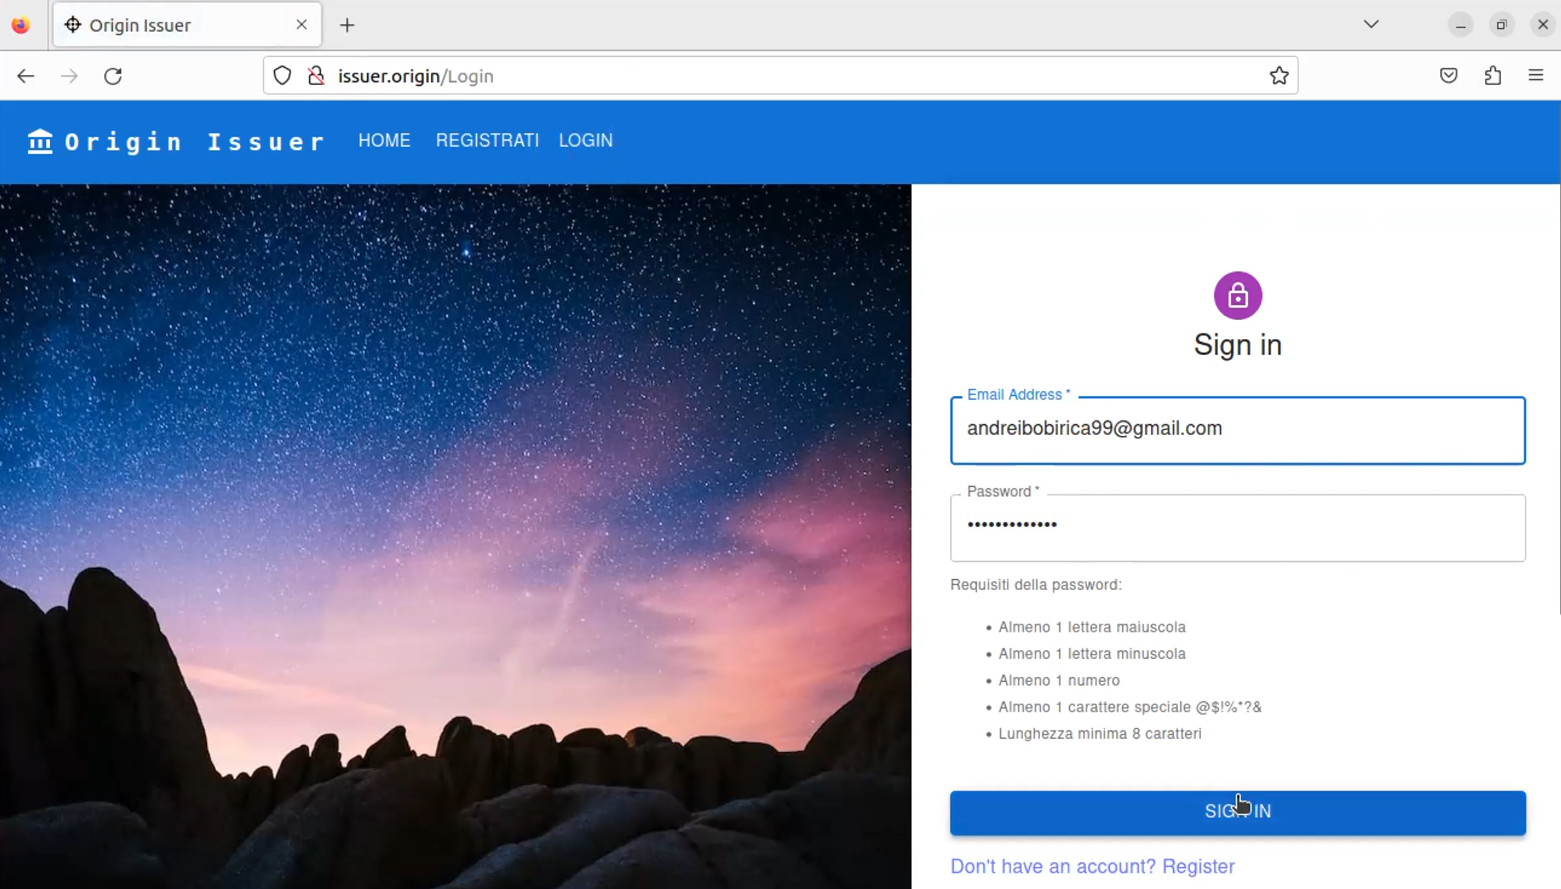
\includegraphics[scale = 0.2]{./res/img/issuer/new/login1.png}
    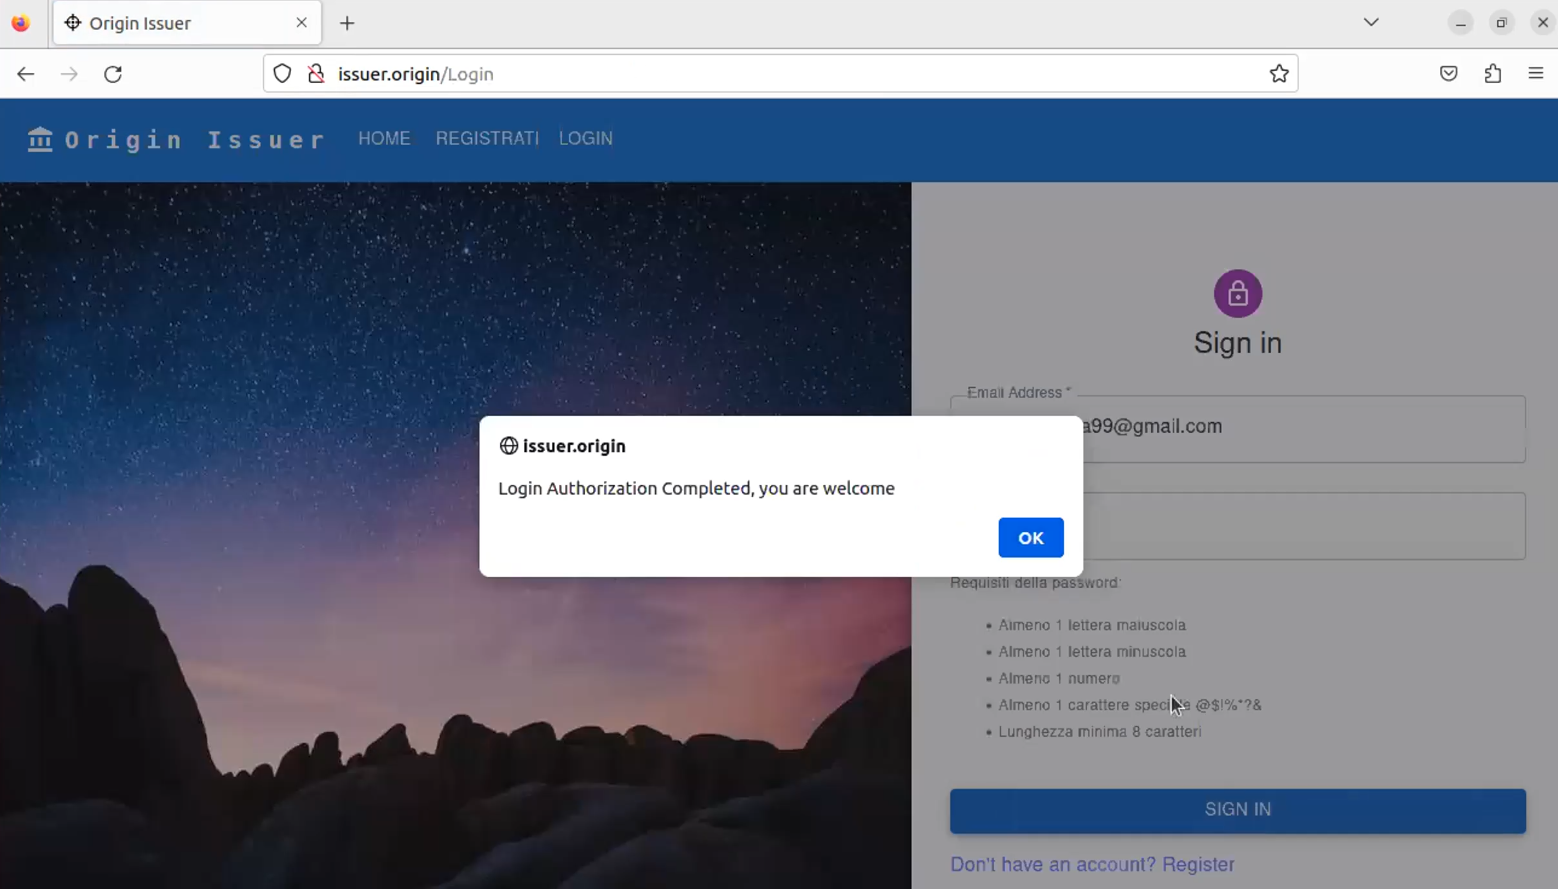
\includegraphics[scale = 0.2]{./res/img/issuer/new/login2.png}
    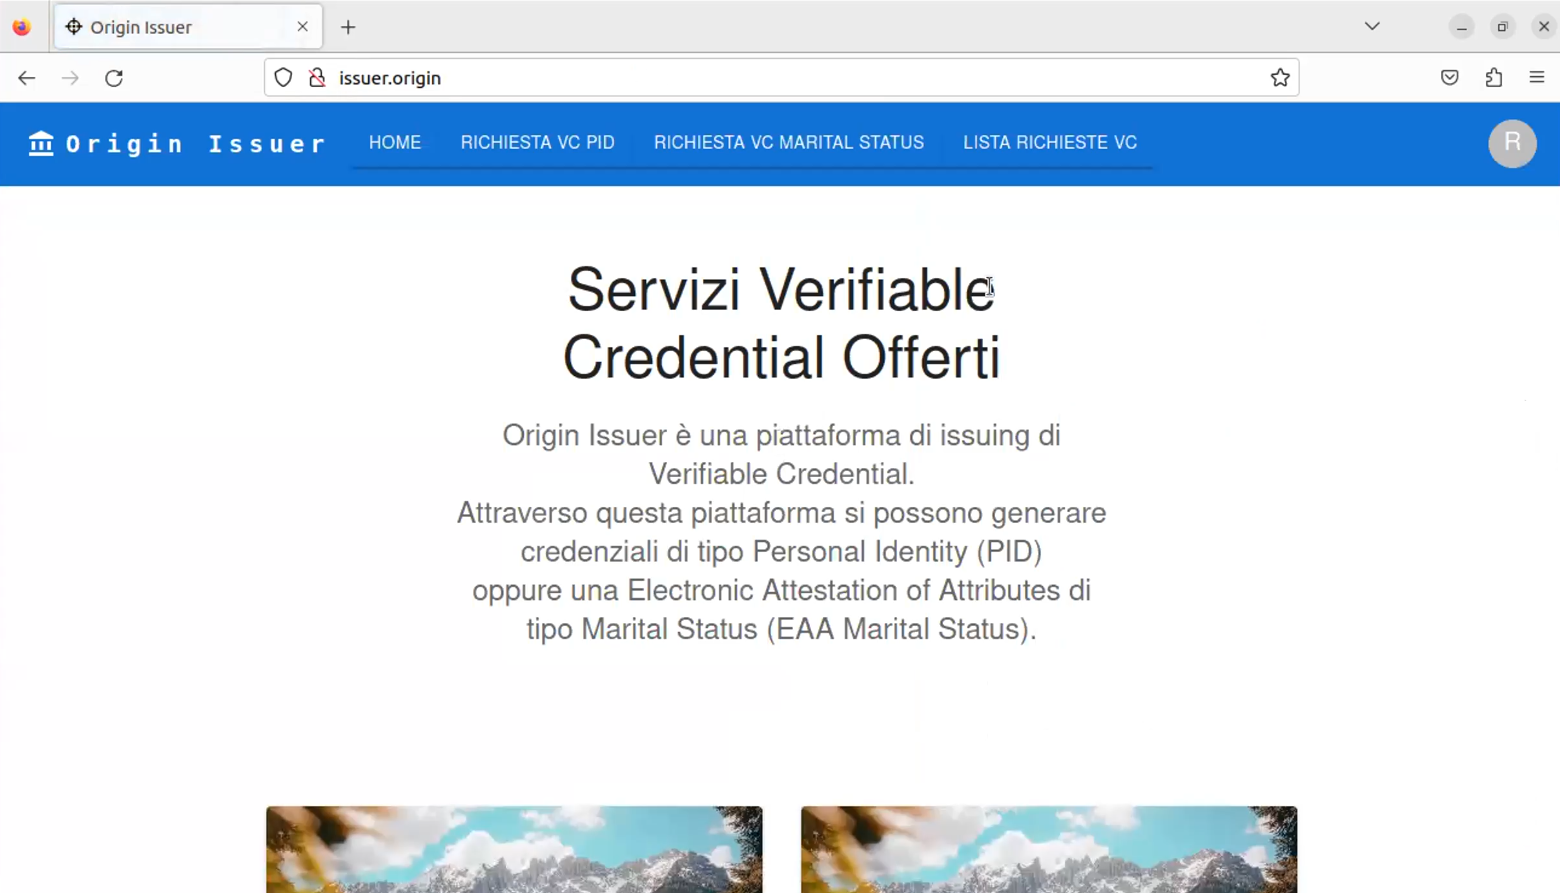
\includegraphics[scale = 0.2]{./res/img/issuer/new/login3.png}
\end{center}



\subsection{Richiesta Credenziale}
\subsubsection{Richiesta PID}
In questa pagina un utente può richiedere una credenziale di tipo \textbf{PID} inserendo i dati richiesti. Una volta inseriti i dati l'utente riceverà un messaggio di conferma e verrà reindirizzato alla lista delle proprie richieste di credenziali.
\begin{center}
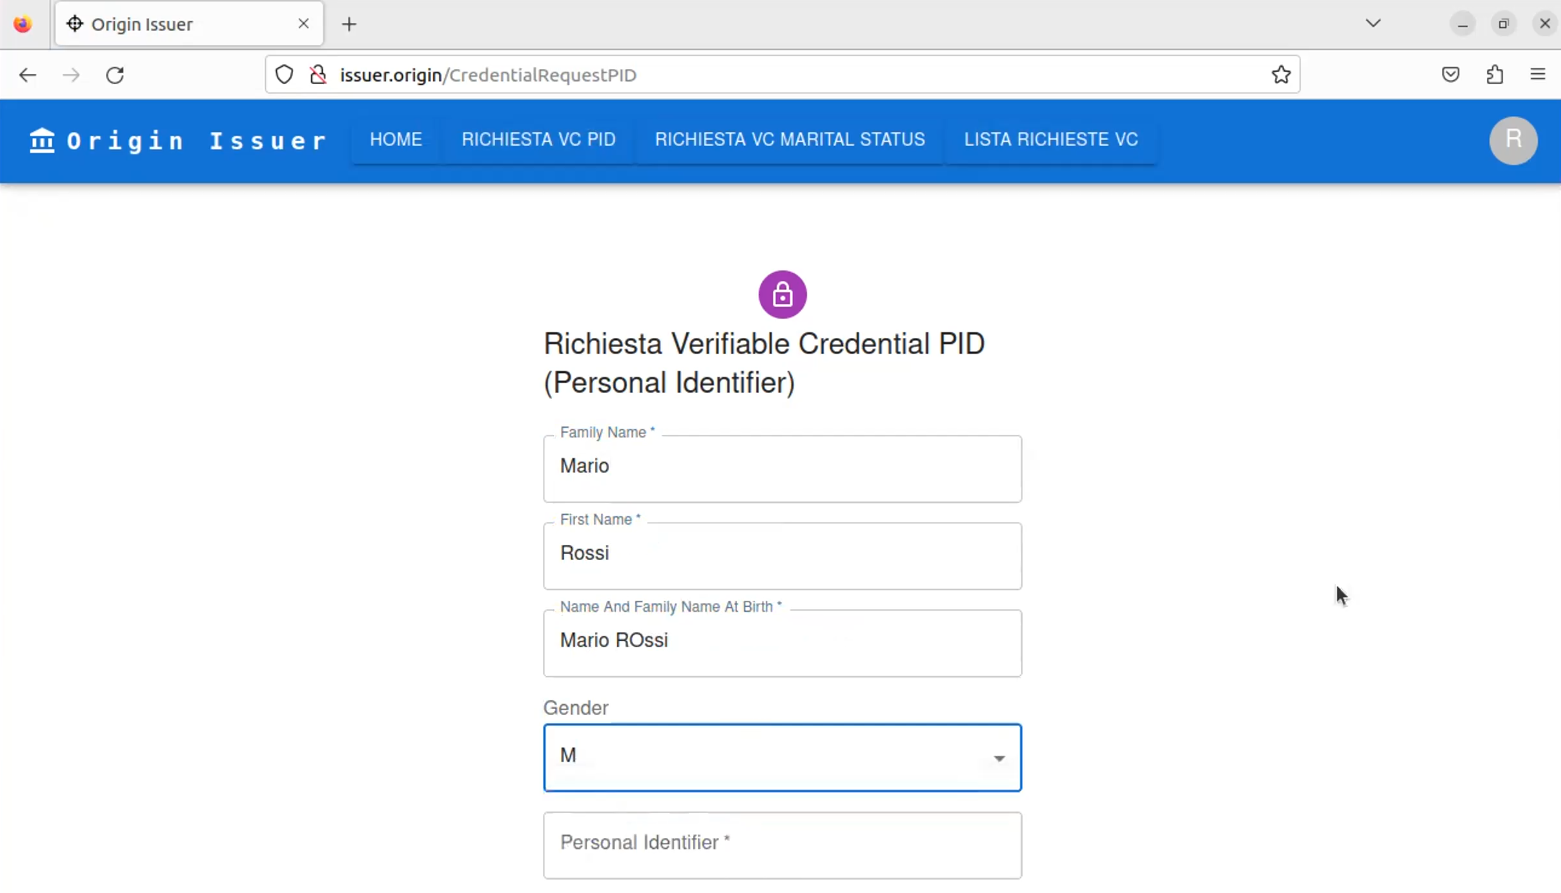
\includegraphics[scale = 0.2]{./res/img/issuer/new/richiestapid1.png}
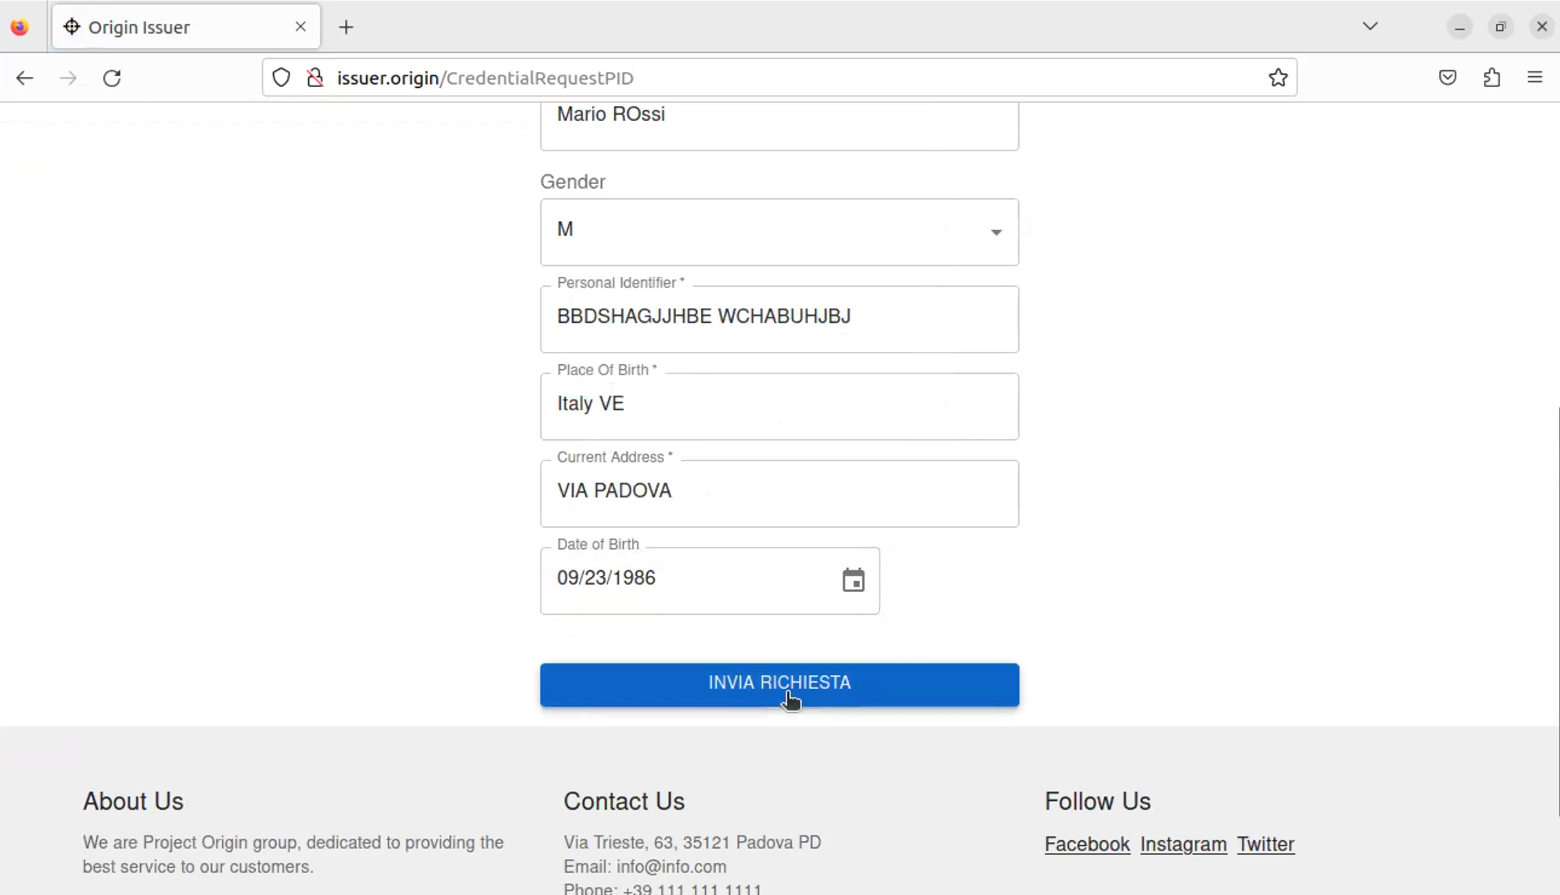
\includegraphics[scale = 0.2]{./res/img/issuer/new/richiestapid2.png}
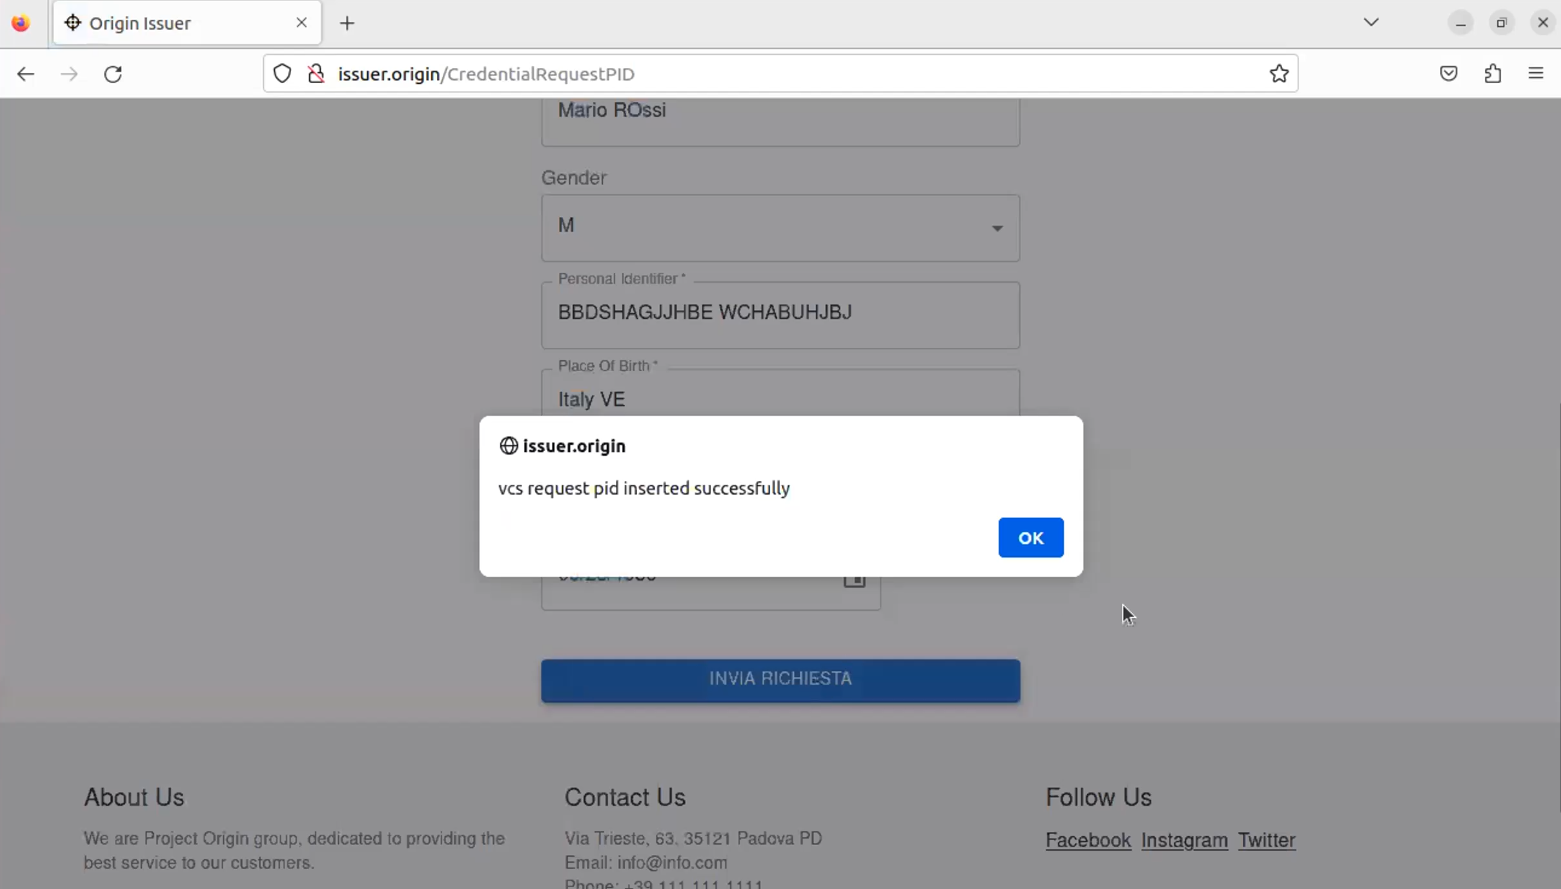
\includegraphics[scale = 0.2]{./res/img/issuer/new/richiestapid3.png}
\end{center}

\subsubsection{Richiesta Marital Status}
In questa pagina un utente può richiedere una credenziale di tipo \textbf{Marital} inserendo i dati richiesti. Una volta inseriti i dati l'utente riceverà un messaggio di conferma e verrà reindirizzato alla lista delle proprie richieste di credenziali.

\subsection{Visualizzazione lista richieste}
\subsubsection{Visualizzazione richieste user} 
In questa pagina l'utente dopo aver fatto una richiesta di credenziale può visualizzare due liste suddivise in PID e Marital. Cliccando su \textbf{Dettaglio} si possono visualizzare tutte le informazioni di una richiesta di credenziale, insieme al suo stato di revisione (In Revisione, Approvato o Rifiutato) e se la credenziale è già stata rilasciata o meno.
\begin{center}
    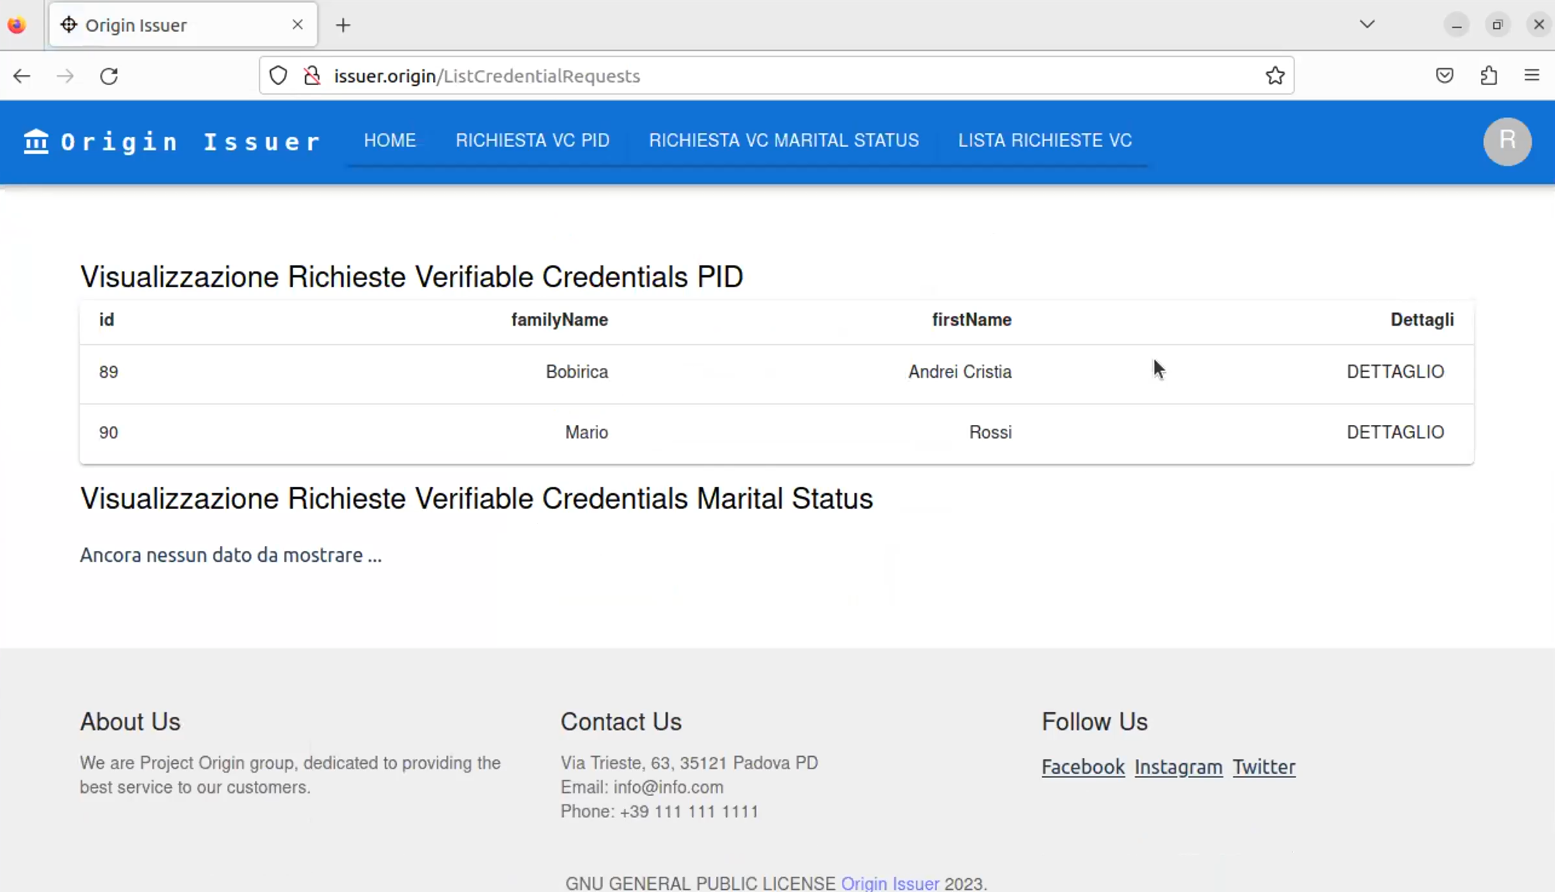
\includegraphics[scale = 0.2]{./res/img/issuer/new/listauser1.png}
    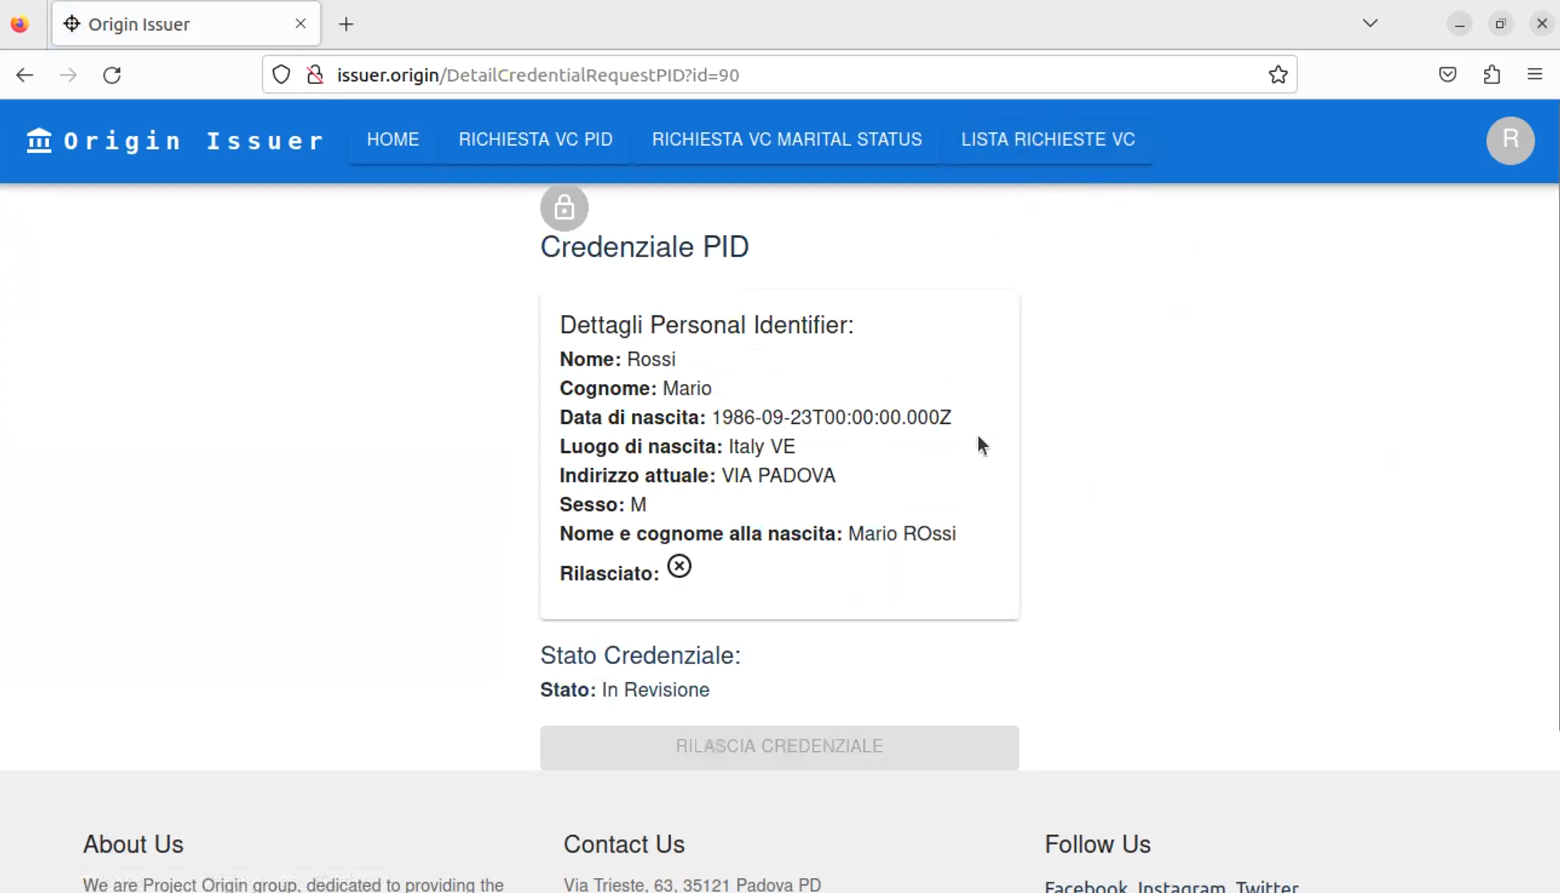
\includegraphics[scale = 0.2]{./res/img/issuer/new/listauser2.png}

\end{center}

\subsection{Rilascio credenziale}
Quando un utente si trova nella pagina di dettaglio di una sua richiesta di credenziale, se la richiesta è stata approvata e la credenziale non è ancora stata rilasciata, l'utente può cliccare sul pulsante Rilascia per rilasciare la credenziale. L'utente può scegliere di rilasciare la credenziale in due maniere: cross device o same device.\\
Inquadrando il codice QR con il proprio wallet si procede con il rilascio in modalità cross device.\\
Per utilizzare la modalità same device si può utilizzare uno dei wallet proposti dall'issuer, come l'Origin Wallet. Successivamente si verrà reindirizzati al wallet.
\begin{center}
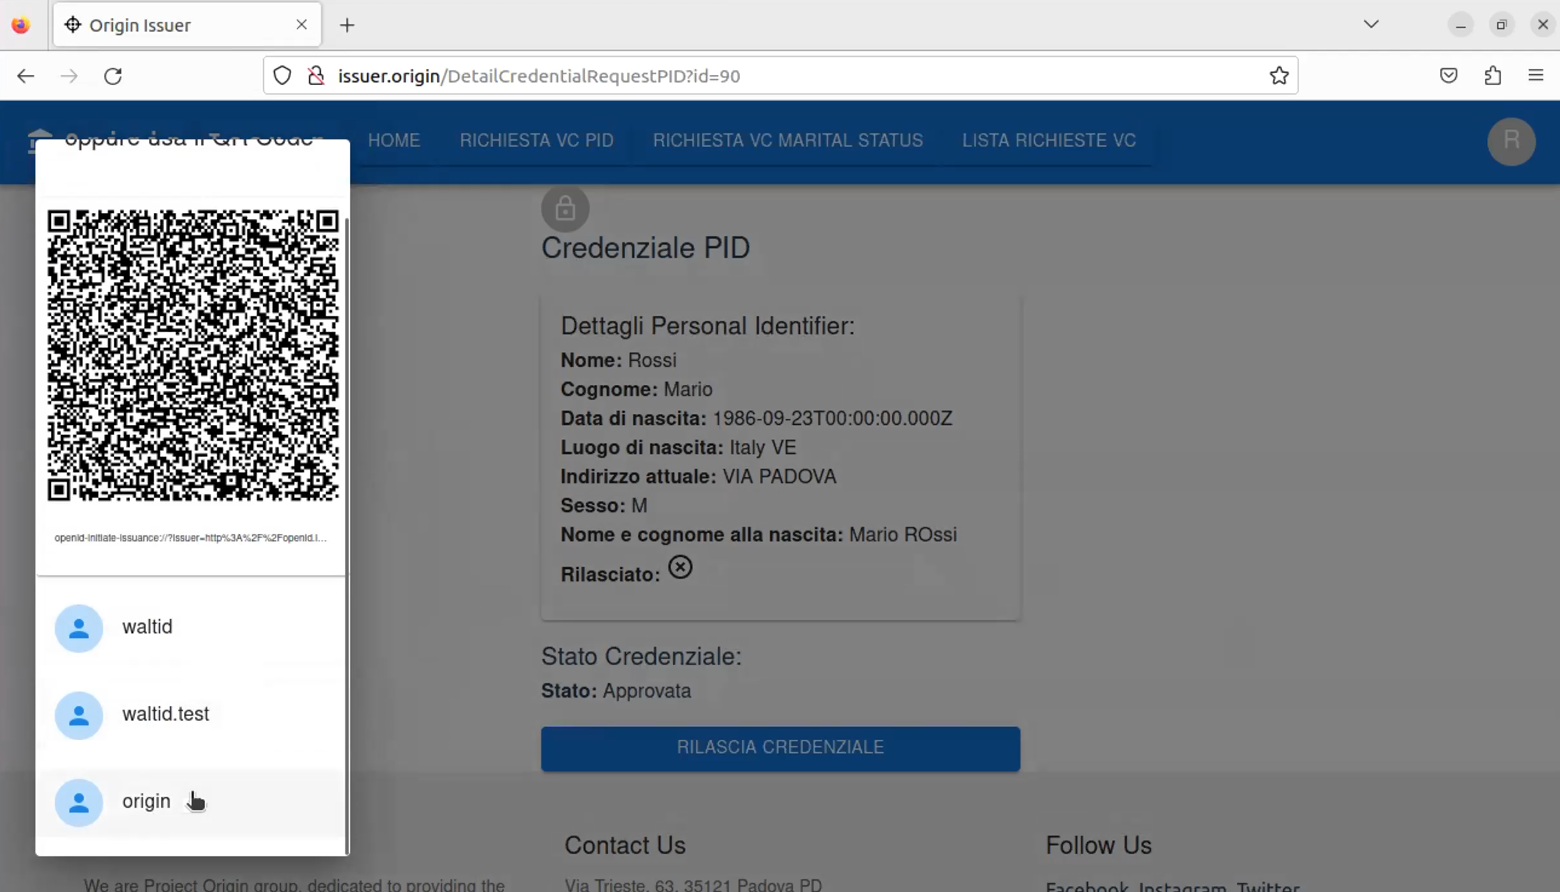
\includegraphics[scale = 0.2]{./res/img/issuer/new/rilascio1.png}  
\end{center}


\subsection{Control Panel Sys Admin}
\subsubsection{Login admin}
In questa pagina un \textbf{admin} può effettuare il login inserendo \textbf{Email} e \textbf{Password} valide. Una volta effettuato il login l'admin verrà reindirizzato alla sua pagina \textbf{Home}.
\begin{center}
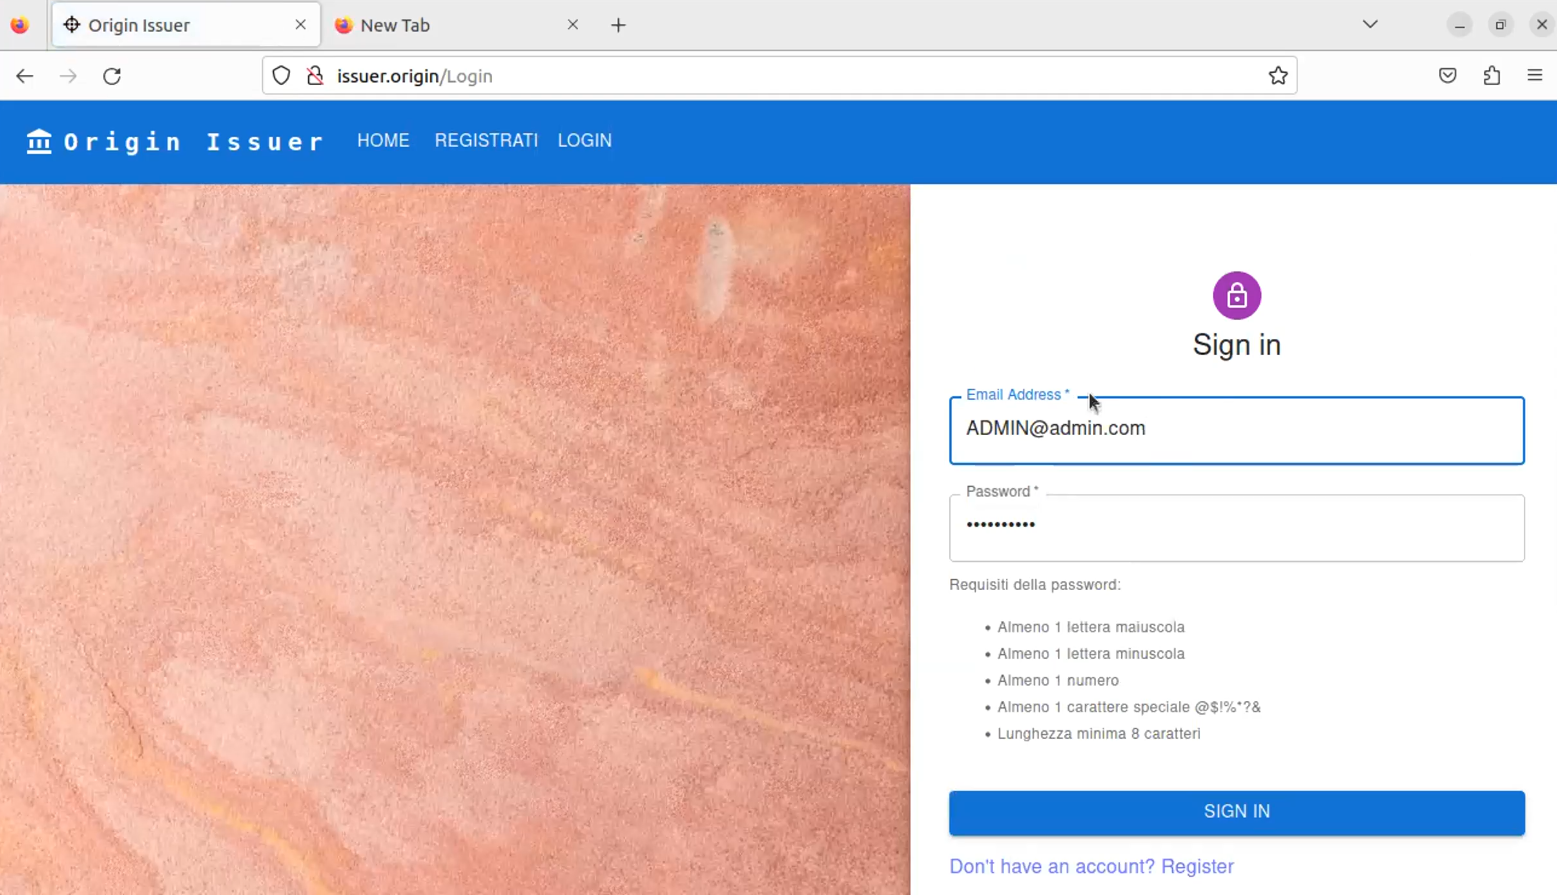
\includegraphics[scale = 0.2]{./res/img/issuer/new/loginadmin1.png}
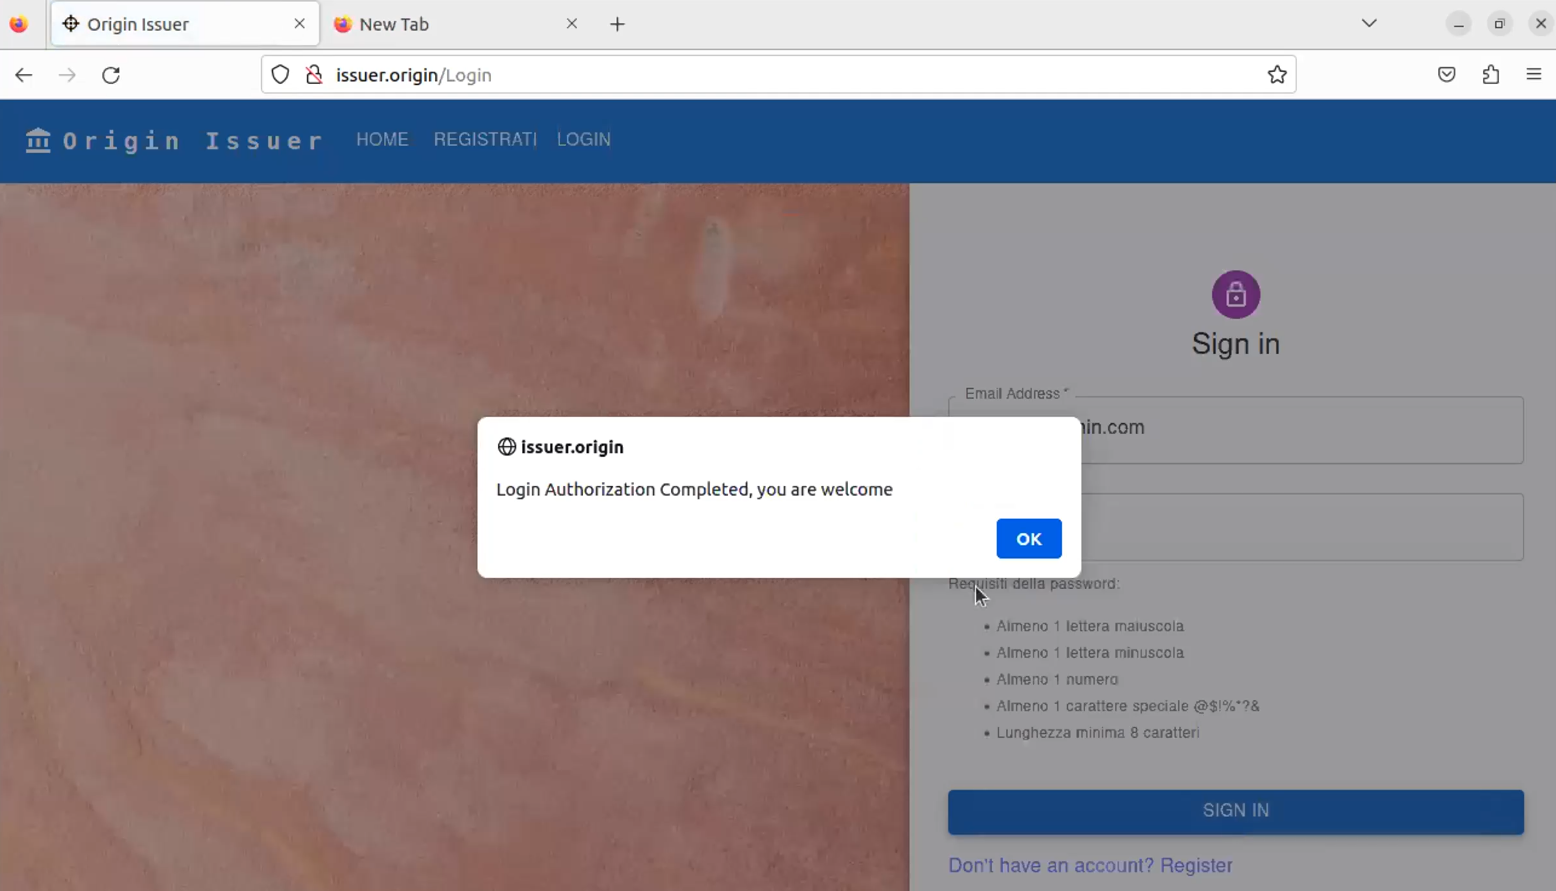
\includegraphics[scale = 0.2]{./res/img/issuer/new/loginadmin2.png}
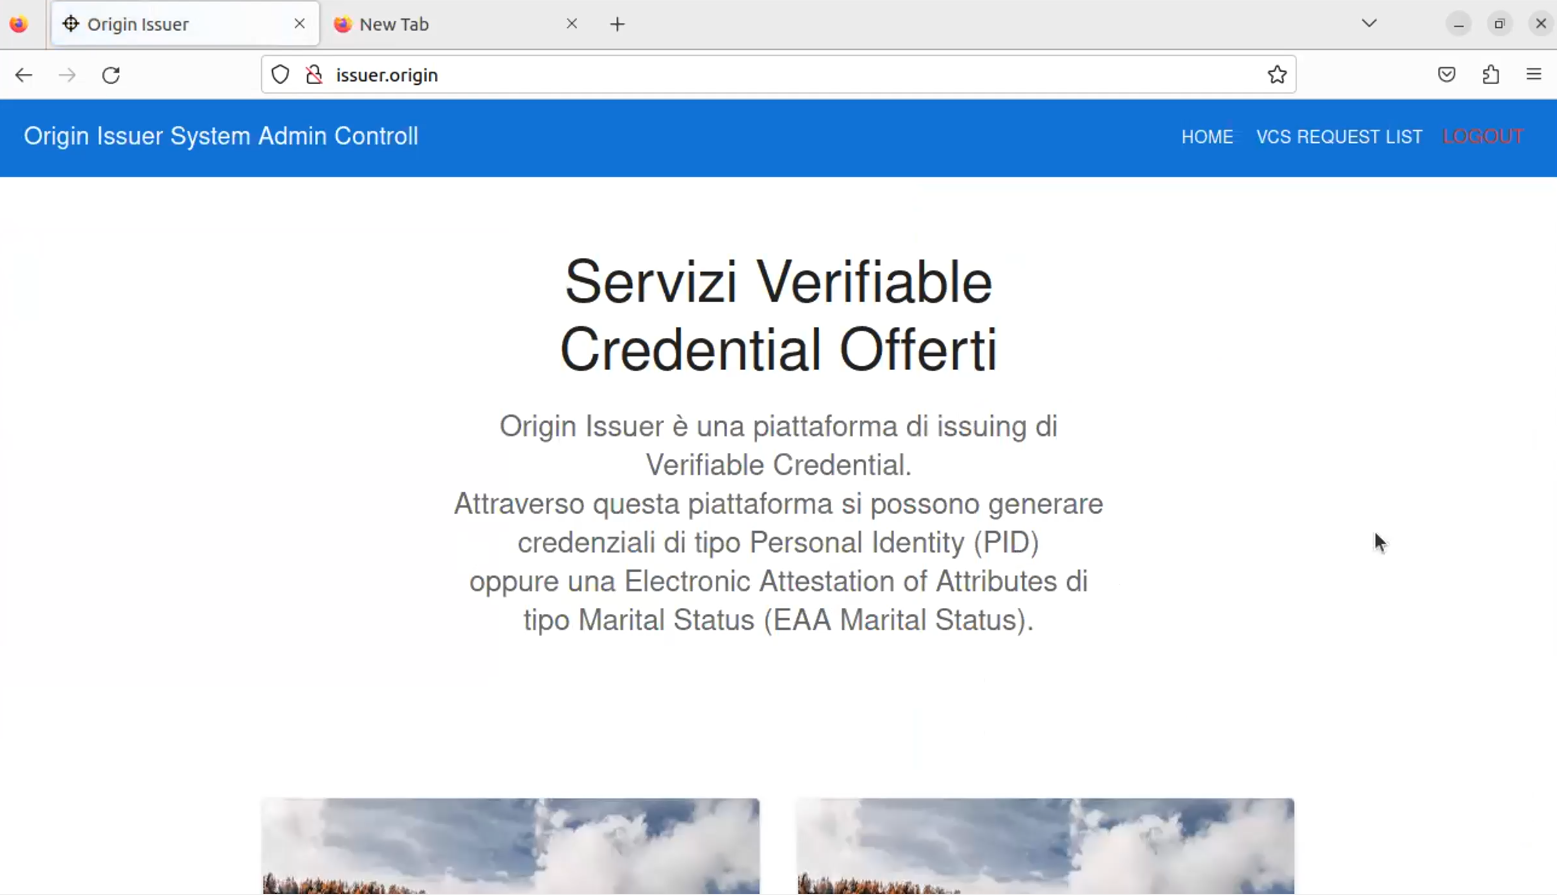
\includegraphics[scale = 0.2]{./res/img/issuer/new/loginadmin3.png}
\end{center}

\subsubsection{Visualizzazione richieste admin e approvazione} 
In questa pagina un admin può visualizzare due liste suddivise in pending e not pending. La lista delle richieste in pending rappresentano le richieste di credenziali non approvate. Cliccando sul pulsante \textbf{Verify} l'admin può approvare o rifiutare la richiesta di credenziale.\\
La lista delle richieste not pending contiene le richieste di credenziali già revisionate, non possono essere modificate.
\begin{center}
    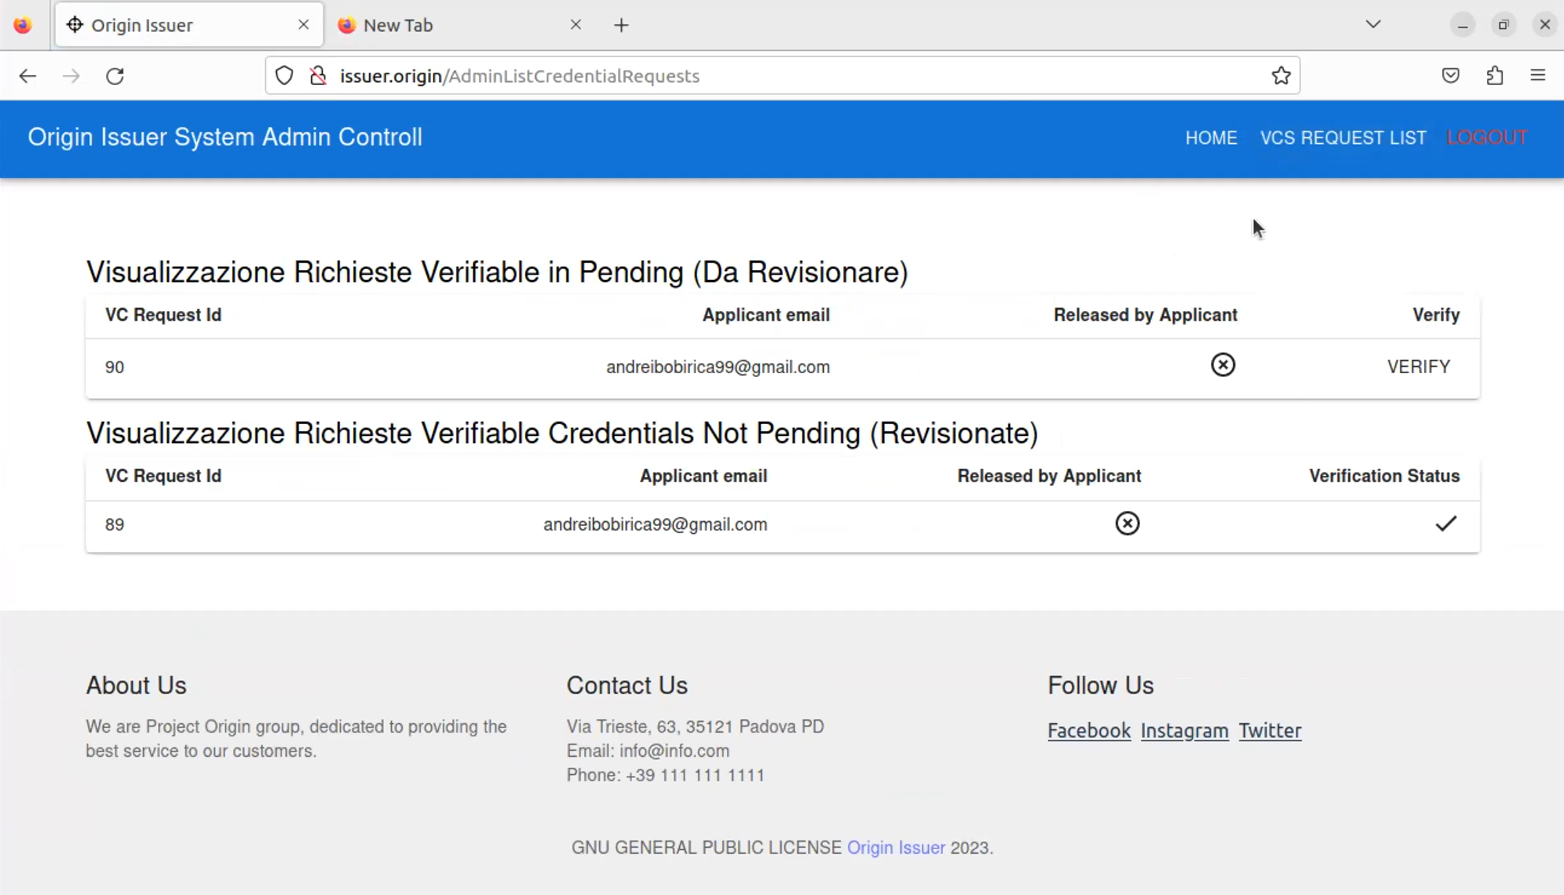
\includegraphics[scale = 0.2]{./res/img/issuer/new/listaadmin1.png}
    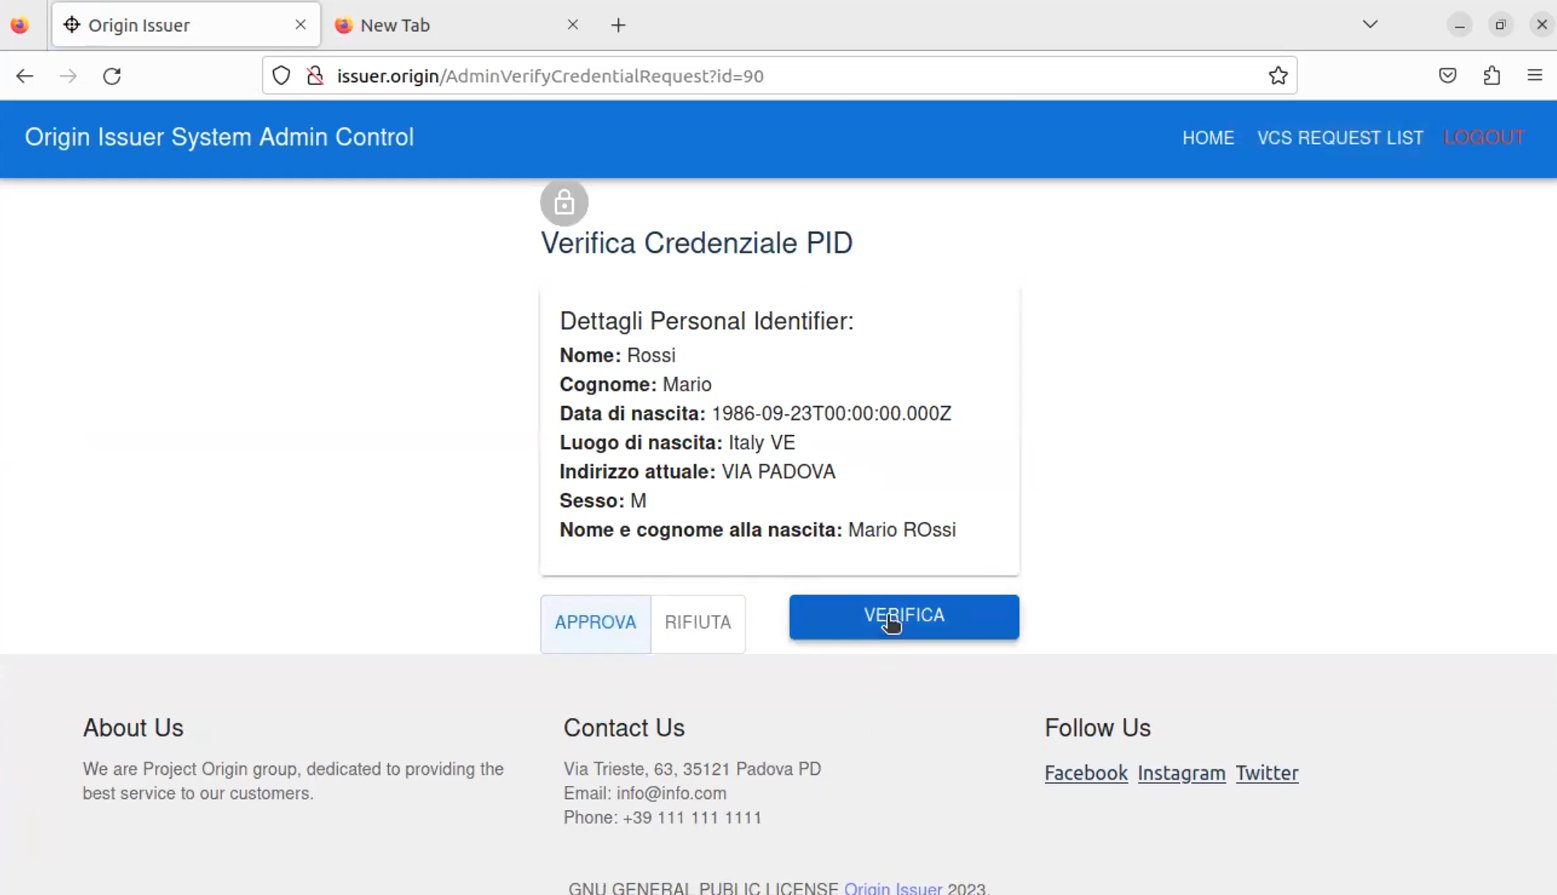
\includegraphics[scale = 0.2]{./res/img/issuer/new/listaadmin2.png}
\end{center}


\clearpage\newpage
\section{Wallet}
Il wallet consente la gestione di credenziali richieste presso un issuer.

\subsection{Registrazione al Wallet}
Per la registrazione occorre fornire un indirizzo email e una password
\begin{center}
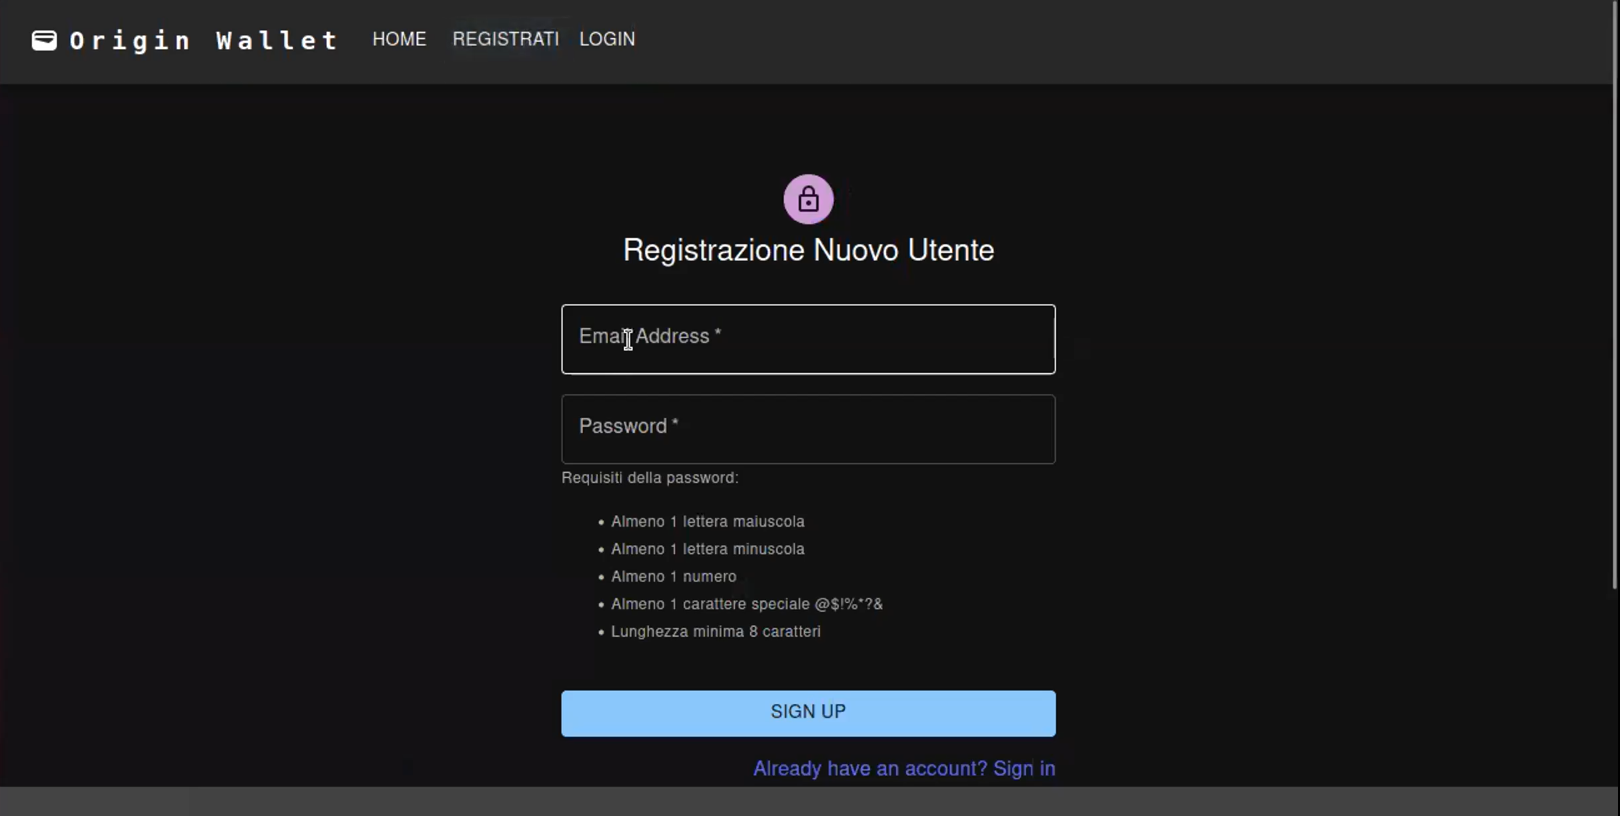
\includegraphics[scale = 0.9]{./res/img/wallet/wallet_register.png}
\end{center}

\subsection{Login al Wallet}
Il login si effettua utilizzando email e password utilizzate durante la registrazione

\subsection{Storage di credenziale}
Una volta effettuato il login al wallet e richiesto il Rilascio di una credenziale presso un issuer, è possibile concludere il processo di Issuing cliccando su Accept.\\
In questo modo la credenziale verrà memorizzata nel wallet
\begin{center}
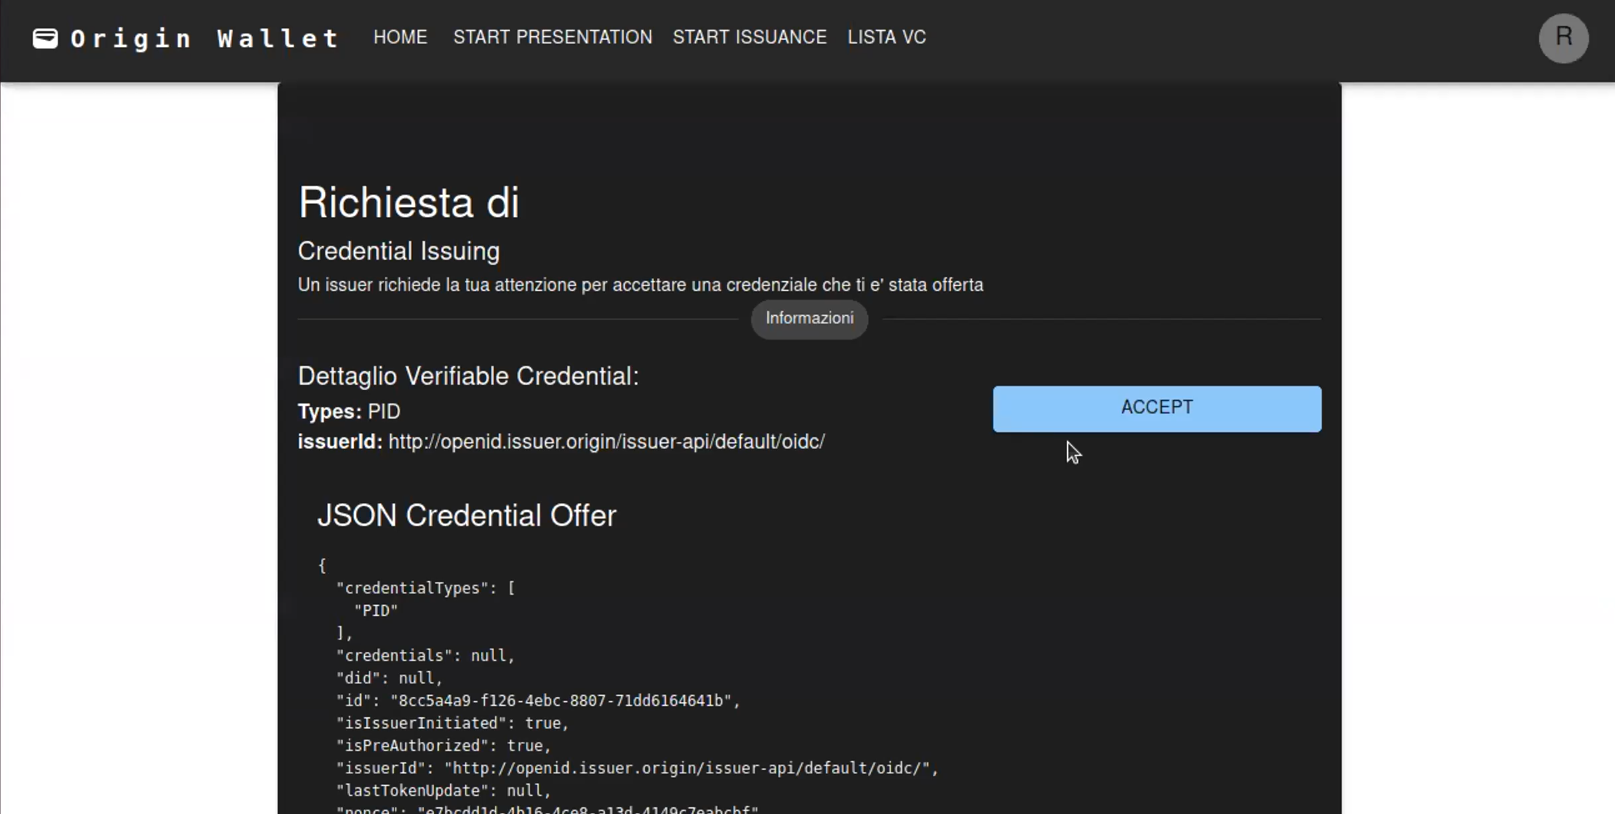
\includegraphics[scale = 0.9]{./res/img/wallet/wallet_continue_issuing.png}
\end{center}

\subsection{Presentazione di credenziale}
Cliccando su START PRESENTATION è possibile presentare una credenziale ad un verifier per poter accedere a dei servizi
\begin{center}
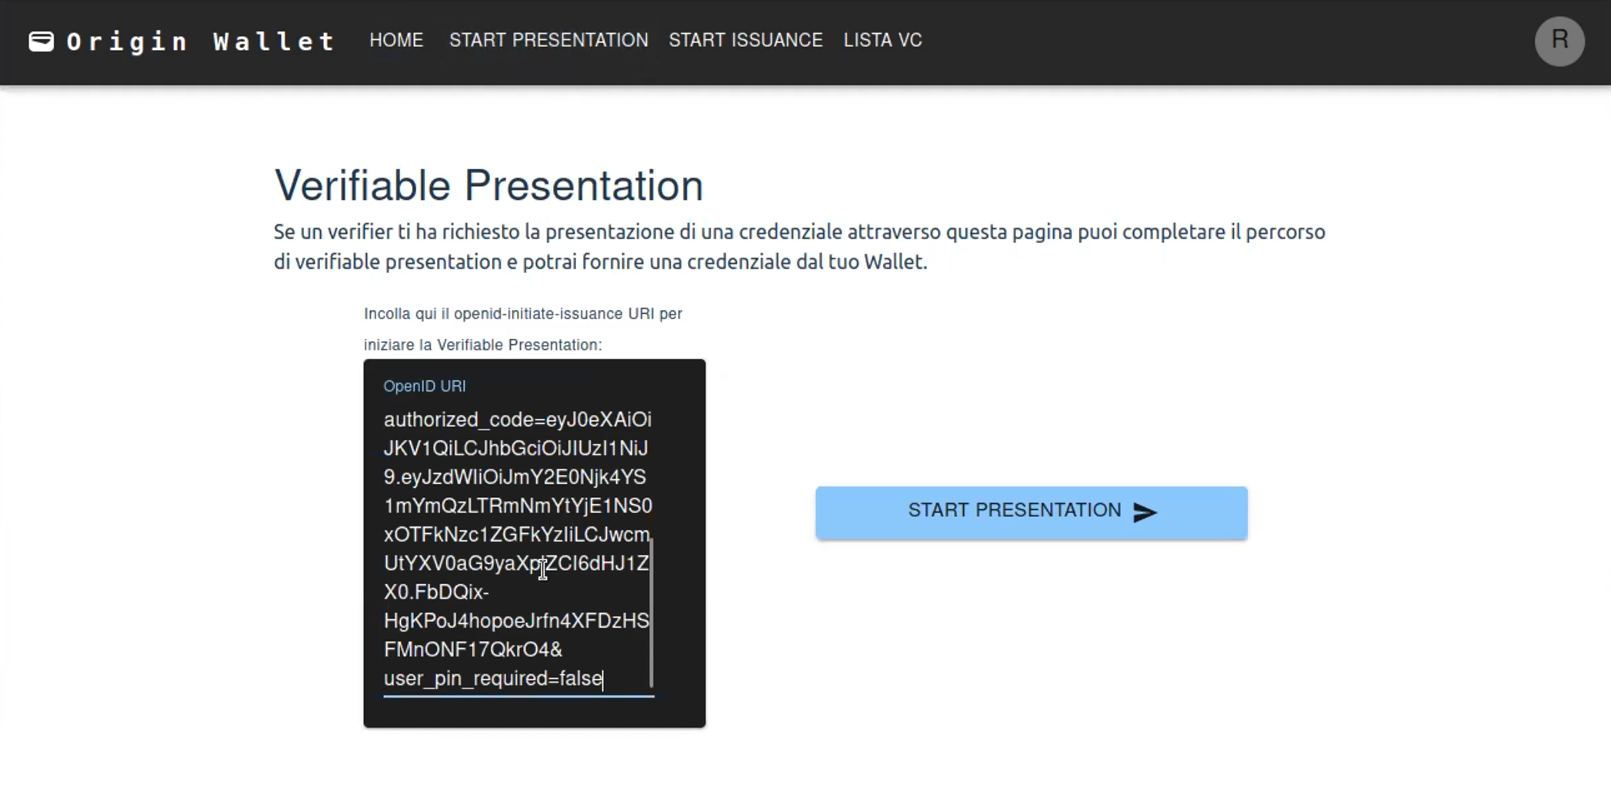
\includegraphics[scale = 0.9]{./res/img/wallet/wallet_start_presentation.png}
\end{center}
\subsection{Visualizzazione e gestione}
Nella pagina di visualizzazione verrà mostrato un elenco di tutte le credenziali memorizzate nel wallet. \newline
\begin{center}
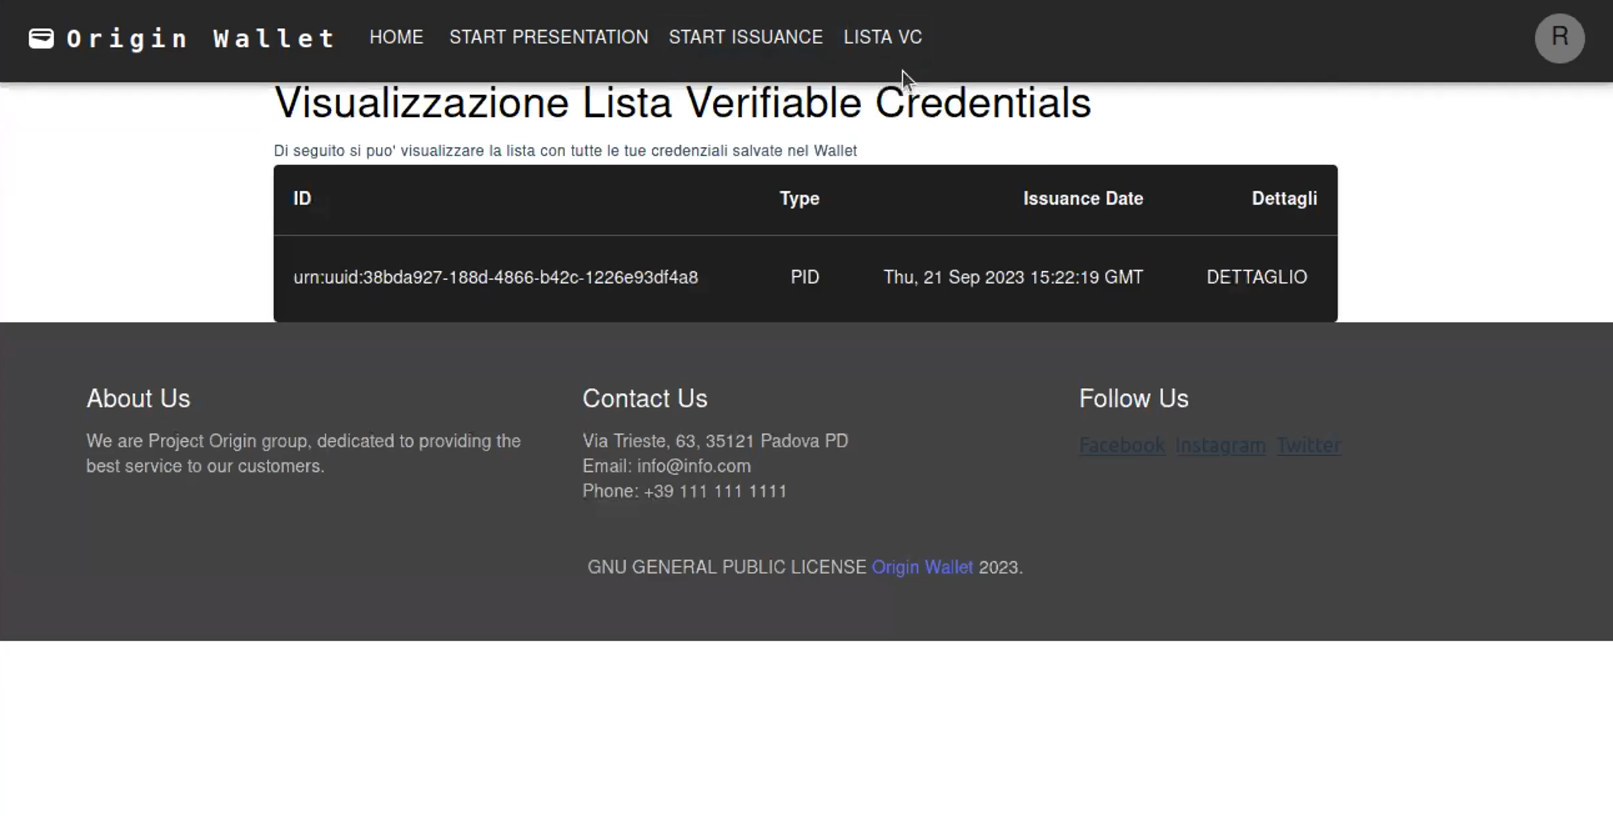
\includegraphics[scale = 0.9]{./res/img/wallet/wallet_credentials_list.png}
\end{center}
Cliccando su DETTAGLIO è possibile visualizzare tutte le informazioni memorizzate nella credenziale. \\
\begin{center}
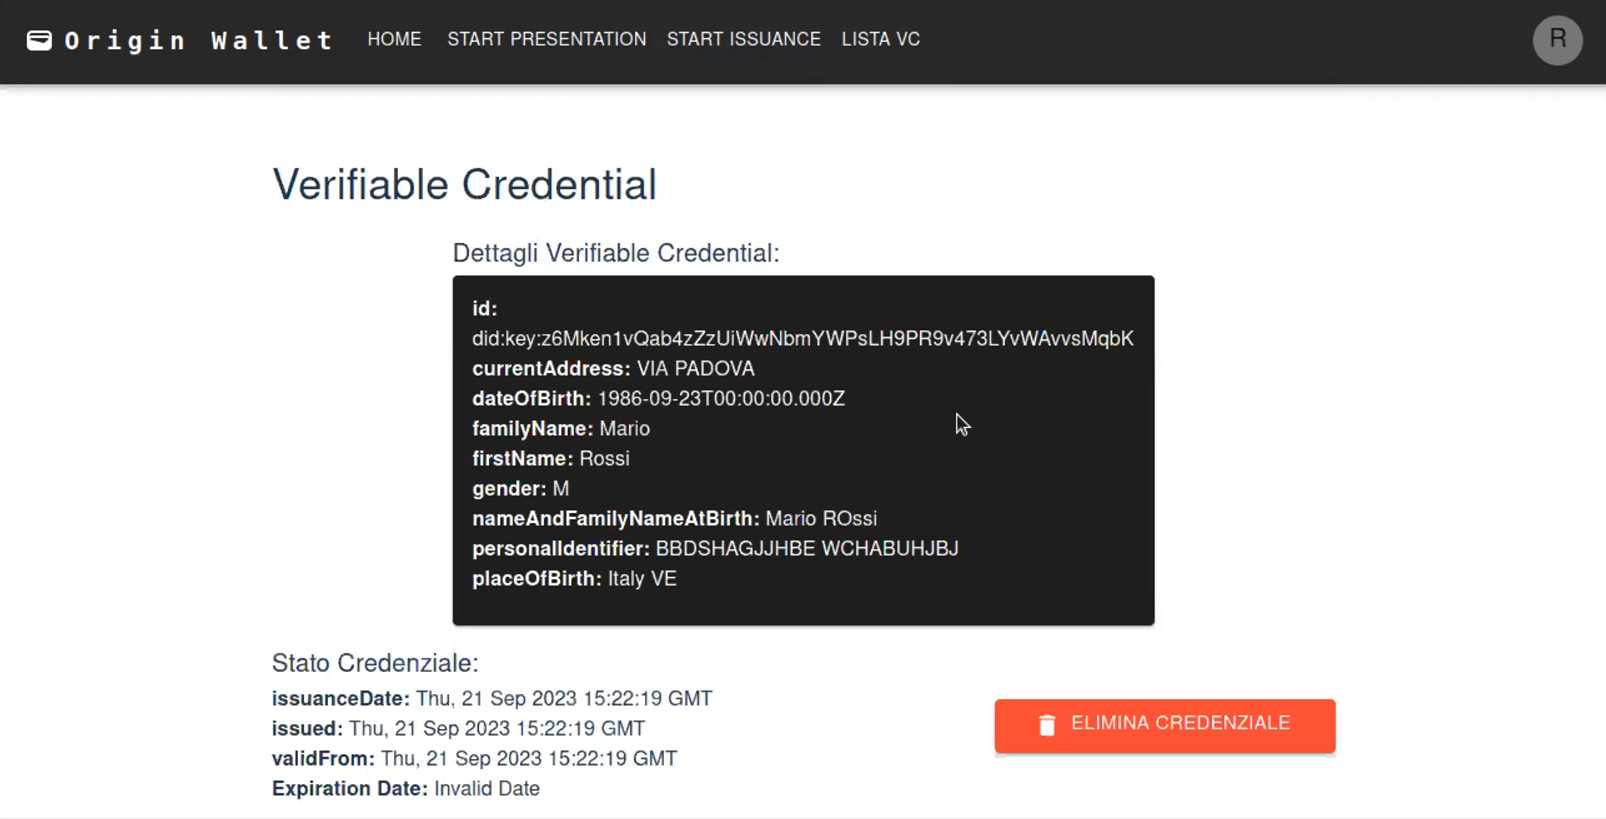
\includegraphics[scale = 0.9]{./res/img/wallet/wallet_credential_detail.png}
\end{center}
In seguito è possibile visualizzate tutte le informazioni contenute in una credenziale, e si può decidere di eliminarla.
\begin{center}
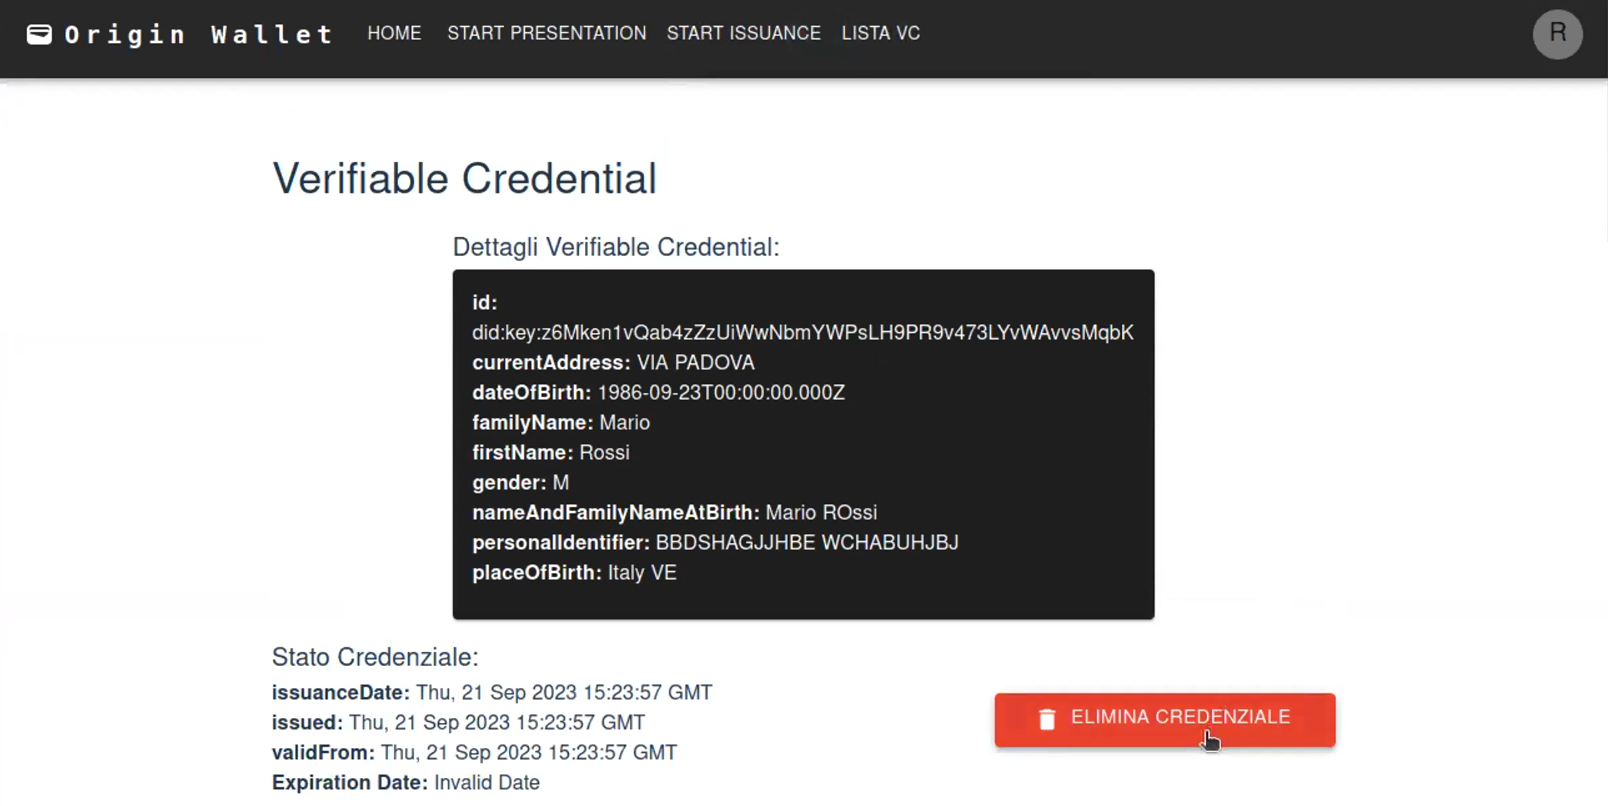
\includegraphics[scale = 0.9]{./res/img/wallet/wallet_credential_delete.png}
\end{center}
%anche se questa immagine è quasi identica a quella di prima, la lascerei\newpage
\section{Verifier}
Il Verifier è un ente che offre dei servizi. Nel nostro esempio è un CAF che offre servizi come la richiesta ISEE.\\
Per accedere a questi servizi la connessione viene effettuata tramite la presentazione di una credenziale di tipo PID.
\subsection{Home}
Per accedere ai servizi offerti bisogna prima effettuare la presentazione di una PID ed effettuare una connessione al verifier.
\begin{center}
    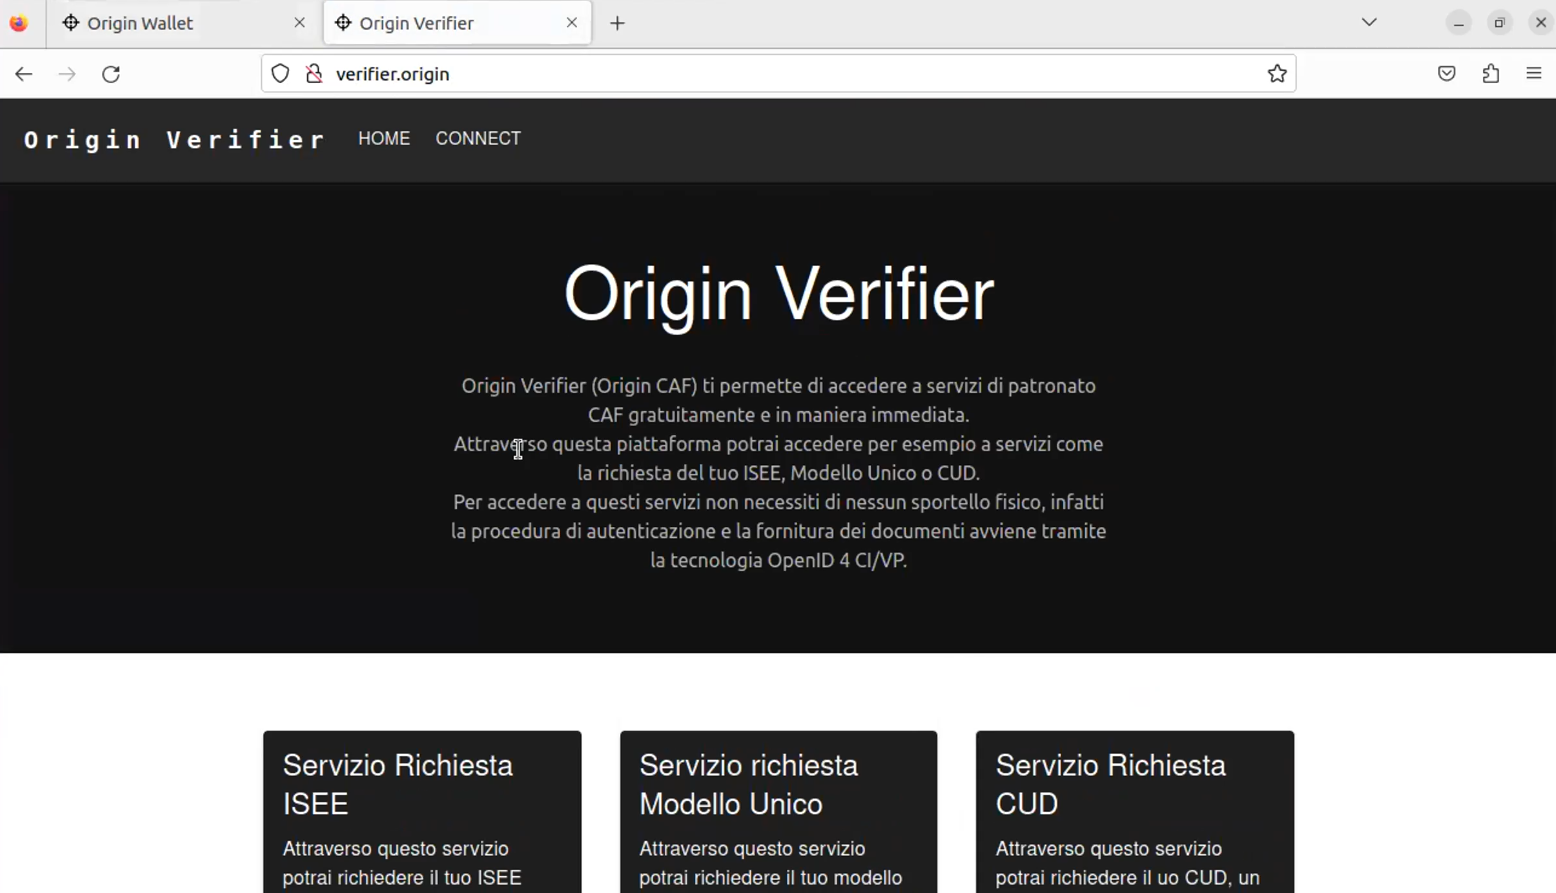
\includegraphics[scale = 0.2]{./res/img/verifier/new/verifier_connect.png}
\end{center}

\subsection{Connessione}
Per accedere ai servizi bisogna effettuare una presentazione di credenziale di tipo PID. La presentazione si può effettuare in modo cross device, inquadrando il qr code, oppure same device, premendo sui pulsanti. Successivamente si verrà reindirizzati al wallet, per continuare la presentazione.
\begin{center}
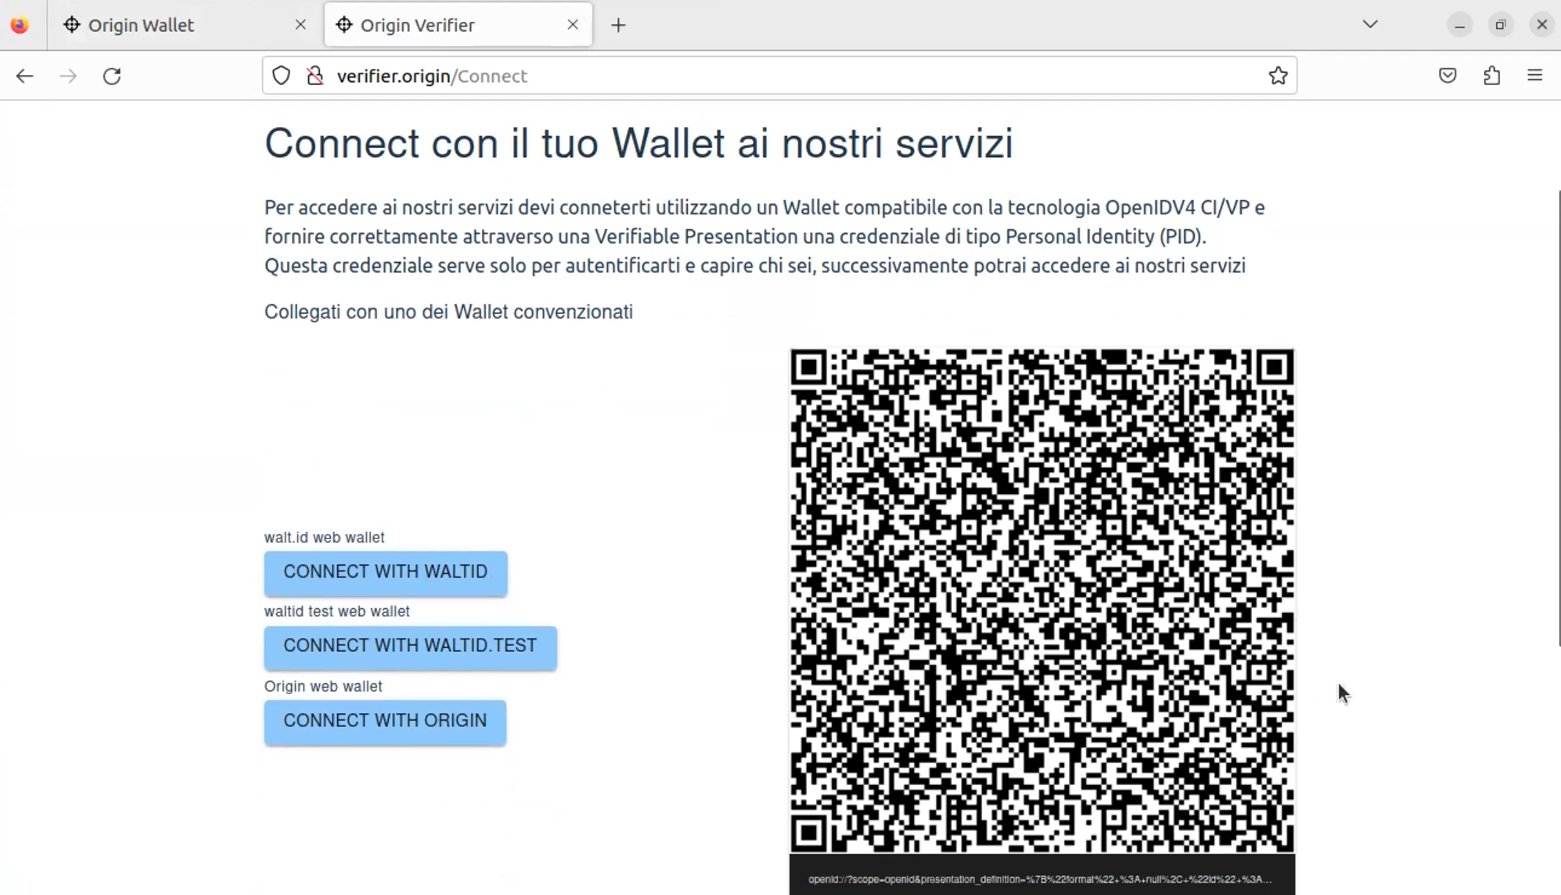
\includegraphics[scale = 0.2]{./res/img/verifier/new/verifier_qr.png}
\end{center}

\subsection{Approvazione presentazione}
Una volta completato da wallet la presentazione di credenziale, si può accettare la presentazione. In particolare si possono visualizzare altri dettagli, come le policy rispettate e l'esito della presentazione.
\begin{center}
    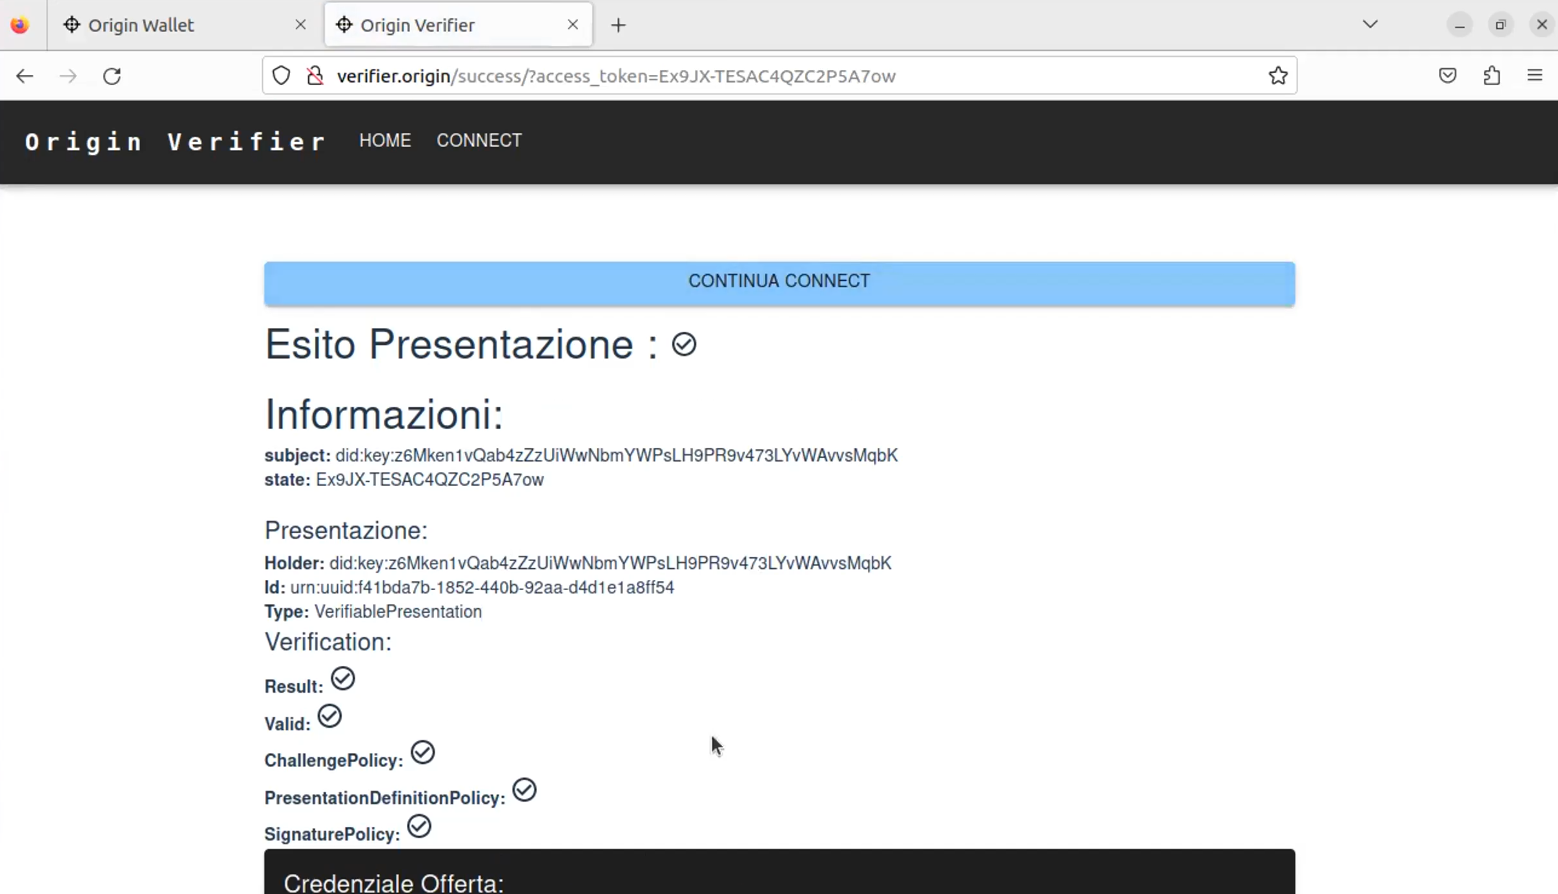
\includegraphics[scale = 0.2]{./res/img/verifier/new/verifier_after_presentation.png}
\end{center}
\subsection{Accesso ai servizi}
Se dalla schermata \textbf{Home} provassimo ad accedere ad un servizio offerto da verifier come in questo caso Servizio isee e l'utente non avesse ancora eseguito la connessione al Wallet e verificato la credenziale necessaria per accedervi, verrà mostrato a schermo un messaggio di errore che cita l'invalidità del token.

\begin{center}
    
    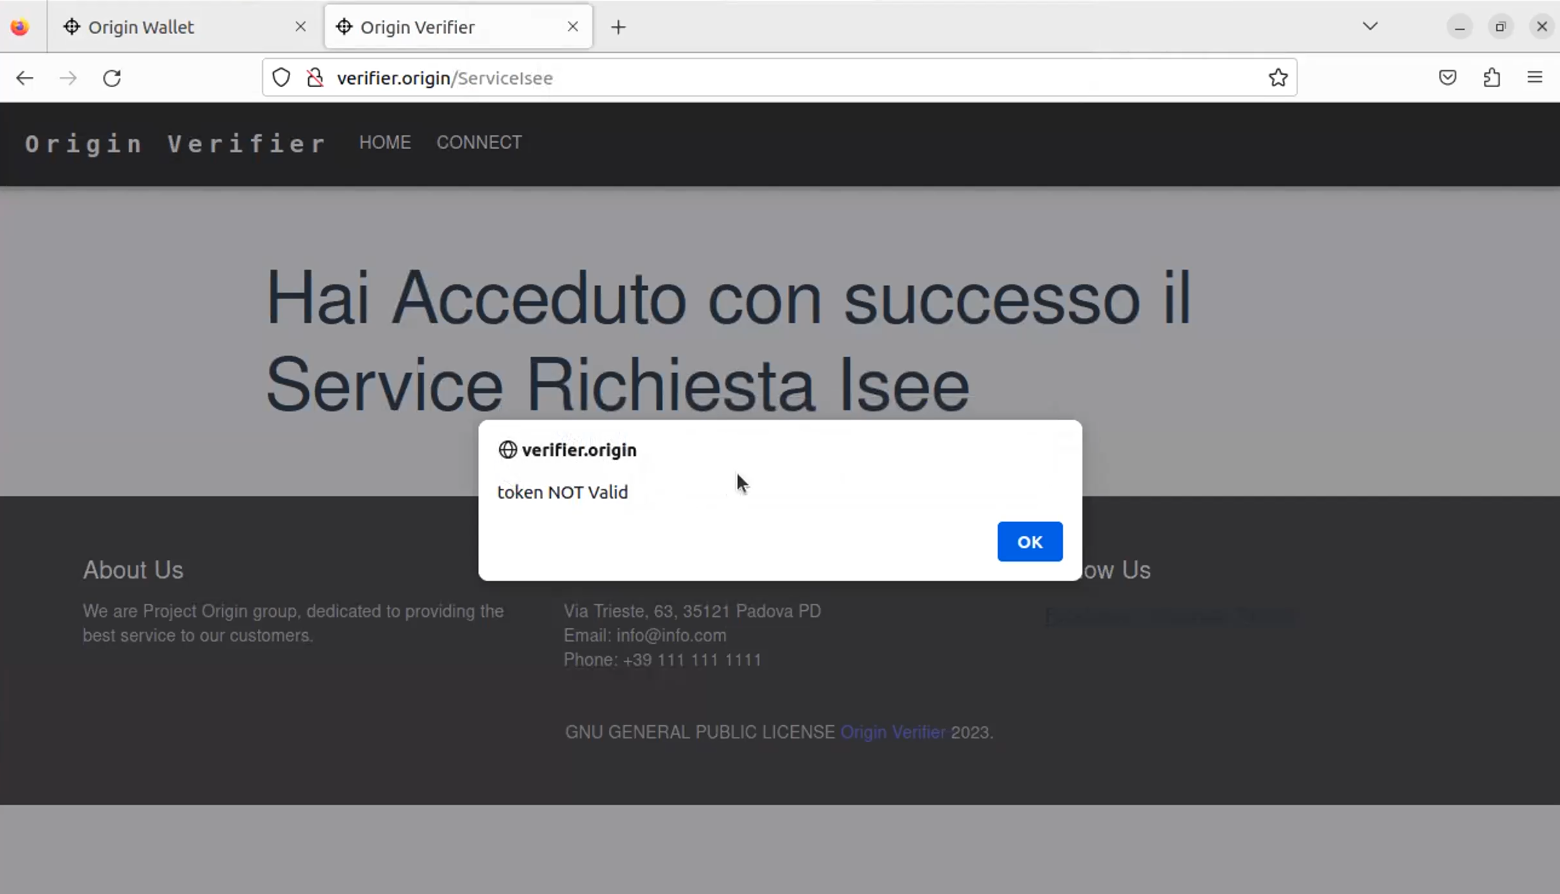
\includegraphics[scale = 0.2]{./res/img/verifier/new/verifier_token_not_valid.png}
\end{center}

Se l'utente avesse completato la  connessione descritta nella sezione precedente può accedere al "Servizio isee" offerto avendo un messaggio di corretto token a disposizione e accedendo correttamente al servizio.\\

\begin{center}
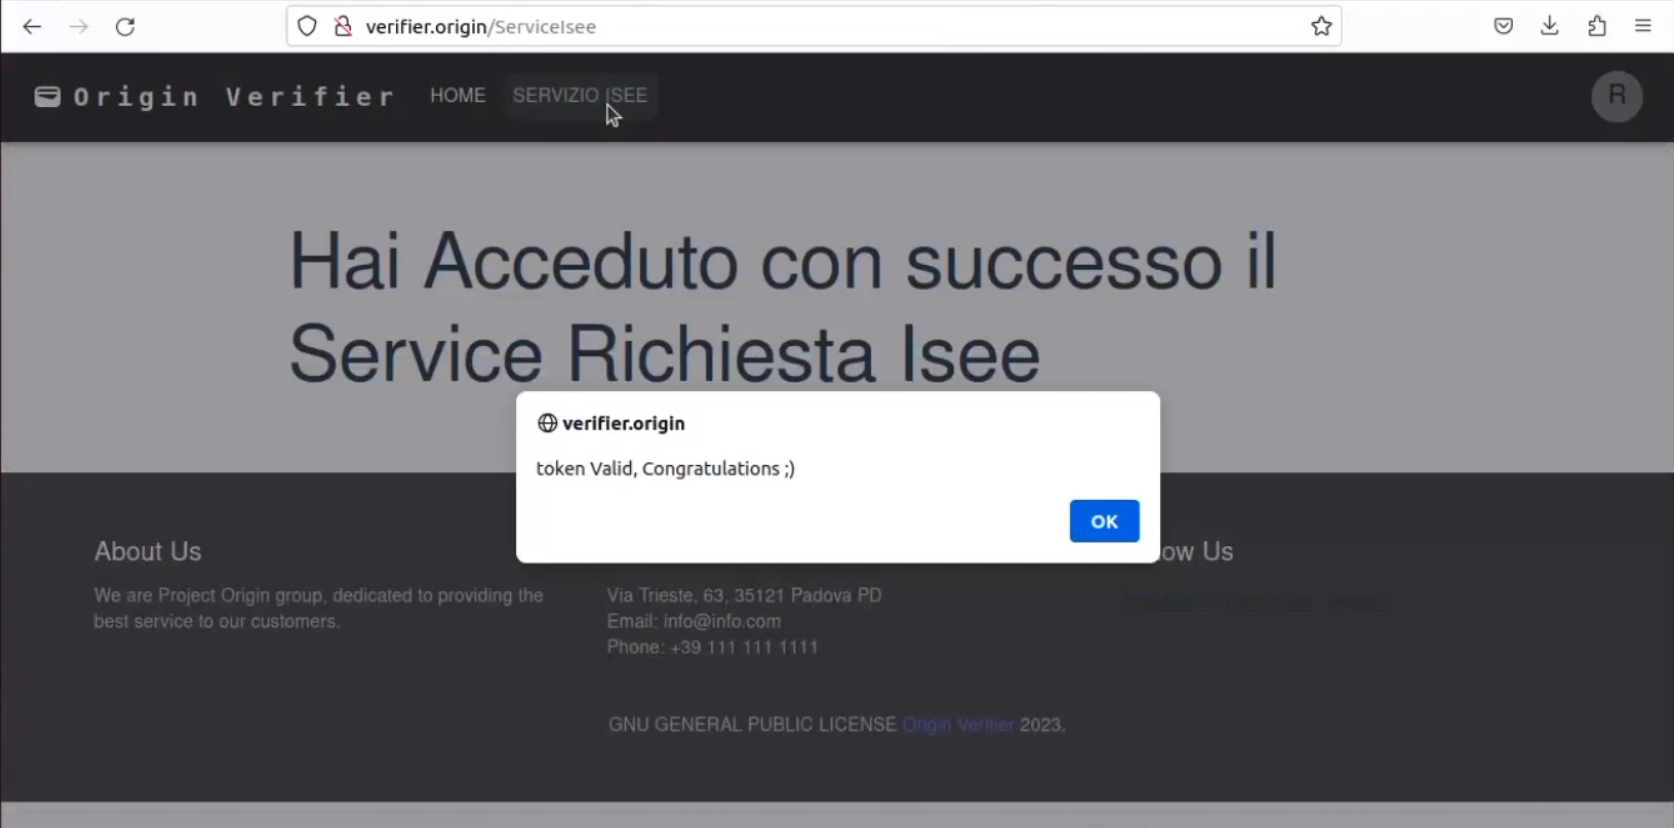
\includegraphics[scale = 0.2]{./res/img/verifier/new/tokenvalido.png}
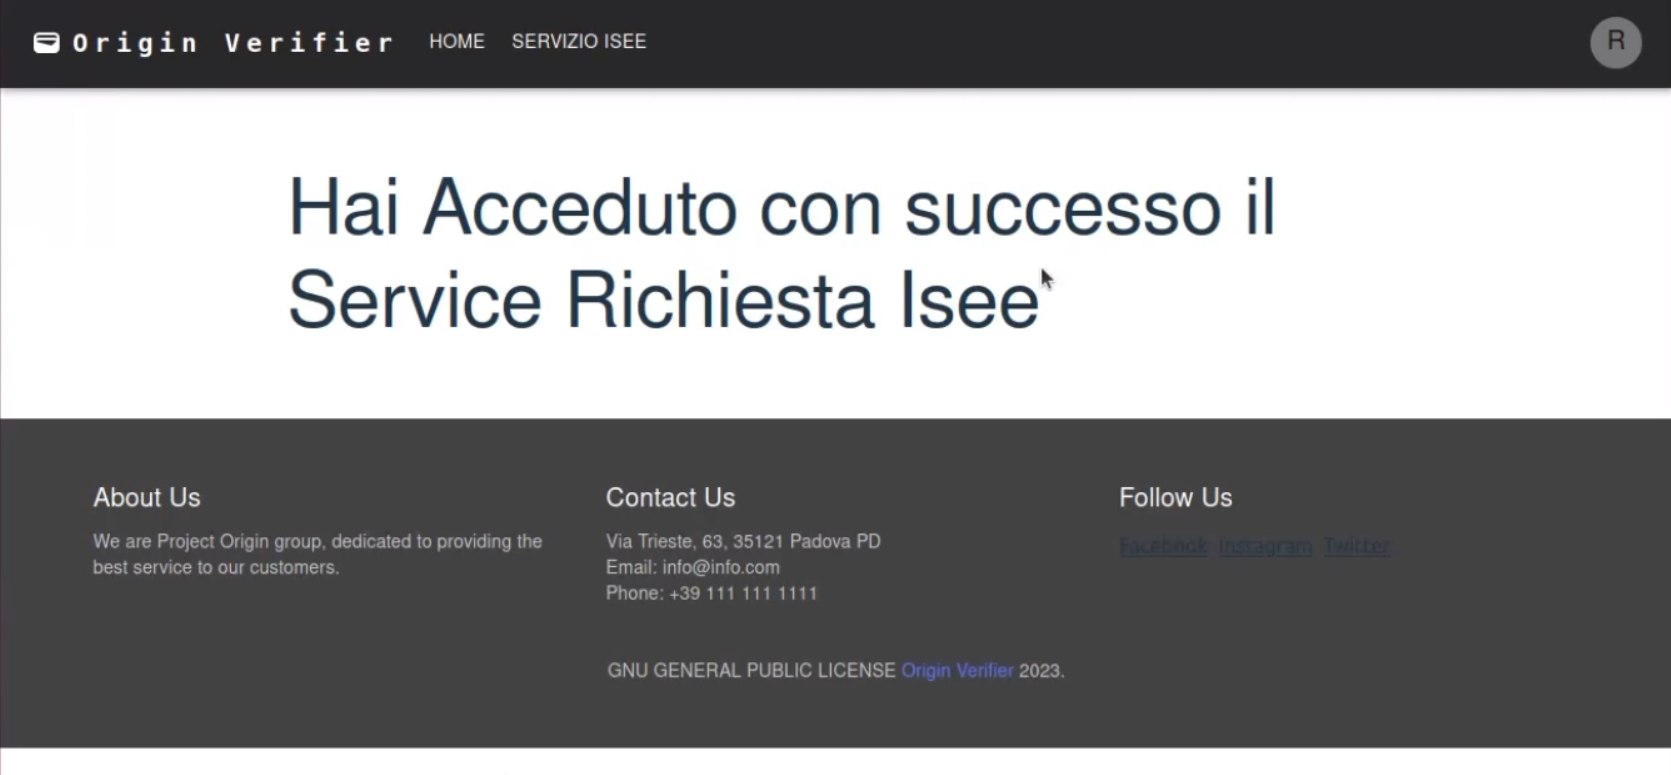
\includegraphics[scale = 0.2]{./res/img/verifier/accessoservizio.png}
\end{center}
\newpage

\pagebreak


\end{document}
